\pdfbookmark{Общая характеристика работы}{characteristic}             % Закладка pdf
\section*{Общая характеристика работы}

\newcommand{\actuality}{\pdfbookmark[1]{Актуальность}{actuality}\underline{\textbf{\actualityTXT}}}
\newcommand{\progress}{\pdfbookmark[1]{Разработанность темы}{progress}\underline{\textbf{\progressTXT}}}
\newcommand{\aim}{\pdfbookmark[1]{Цели}{aim}\underline{{\textbf\aimTXT}}}
\newcommand{\tasks}{\pdfbookmark[1]{Задачи}{tasks}\underline{\textbf{\tasksTXT}}}
\newcommand{\aimtasks}{\pdfbookmark[1]{Цели и задачи}{aimtasks}\aimtasksTXT}
\newcommand{\novelty}{\pdfbookmark[1]{Научная новизна}{novelty}\underline{\textbf{\noveltyTXT}}}
\newcommand{\influence}{\pdfbookmark[1]{Практическая значимость}{influence}\underline{\textbf{\influenceTXT}}}
\newcommand{\methods}{\pdfbookmark[1]{Методология и методы исследования}{methods}\underline{\textbf{\methodsTXT}}}
\newcommand{\defpositions}{\pdfbookmark[1]{Положения, выносимые на защиту}{defpositions}\underline{\textbf{\defpositionsTXT}}}
\newcommand{\reliability}{\pdfbookmark[1]{Достоверность}{reliability}\underline{\textbf{\reliabilityTXT}}}
\newcommand{\probation}{\pdfbookmark[1]{Апробация}{probation}\underline{\textbf{\probationTXT}}}
\newcommand{\contribution}{\pdfbookmark[1]{Личный вклад}{contribution}\underline{\textbf{\contributionTXT}}}
\newcommand{\publications}{\pdfbookmark[1]{Публикации}{publications}\underline{\textbf{\publicationsTXT}}}


{\actuality} Обзор, введение в тему, обозначение места данной работы в
мировых исследованиях и~т.\:п., можно использовать ссылки на другие
работы~\cite{Gosele1999161} (если их нет, то в автореферате
автоматически пропадёт раздел <<Список литературы>>). Внимание! Ссылки
на другие работы в разделе общей характеристики работы можно
использовать только при использовании \verb!biblatex! (из-за технических
ограничений \verb!bibtex8!. Это связано с тем, что одна и та же
характеристика используются и в тексте диссертации, и в
автореферате. В последнем, согласно ГОСТ, должен присутствовать список
работ автора по теме диссертации, а \verb!bibtex8! не умеет выводить в одном
файле два списка литературы).

 \aim\ данной работы является \ldots

Для~достижения поставленной цели необходимо было решить следующие {\tasks}:
\begin{enumerate}
  \item Исследовать, разработать, вычислить и~т.\:д. и~т.\:п.
  \item Исследовать, разработать, вычислить и~т.\:д. и~т.\:п.
  \item Исследовать, разработать, вычислить и~т.\:д. и~т.\:п.
  \item Исследовать, разработать, вычислить и~т.\:д. и~т.\:п.
\end{enumerate}

\defpositions
\begin{enumerate}
  \item Первое положение
  \item Второе положение
  \item Третье положение
  \item Четвертое положение
\end{enumerate}

\novelty
\begin{enumerate}
  \item Впервые \ldots
  \item Впервые \ldots
  \item Было выполнено оригинальное исследование \ldots
\end{enumerate}

\influence\ \ldots

\reliability\ полученных результатов обеспечивается \ldots \ Результаты находятся в соответствии с результатами, полученными другими авторами.

\probation\
Основные результаты работы докладывались~на:
перечисление основных конференций, симпозиумов и~т.\:п.

\contribution\ Автор принимал активное участие \ldots

%\publications\ Основные результаты по теме диссертации изложены в ХХ печатных изданиях~\cite{Sokolov,Gaidaenko,Lermontov,Management},
%Х из которых изданы в журналах, рекомендованных ВАК~\cite{Sokolov,Gaidaenko}, 
%ХХ --- в тезисах докладов~\cite{Lermontov,Management}.

\ifthenelse{\equal{\thebibliosel}{0}}{% Встроенная реализация с загрузкой файла через движок bibtex8
    \publications\ Основные результаты по теме диссертации изложены в XX печатных изданиях, 
    X из которых изданы в журналах, рекомендованных ВАК, 
    X "--- в тезисах докладов.%
}{% Реализация пакетом biblatex через движок biber
%Сделана отдельная секция, чтобы не отображались в списке цитированных материалов
    \begin{refsection}%
        \printbibliography[heading=countauthornotvak, env=countauthornotvak, keyword=biblioauthornotvak, section=1]%
        \printbibliography[heading=countauthorvak, env=countauthorvak, keyword=biblioauthorvak, section=1]%
        \printbibliography[heading=countauthorconf, env=countauthorconf, keyword=biblioauthorconf, section=1]%
        \printbibliography[heading=countauthor, env=countauthor, keyword=biblioauthor, section=1]%
        \publications\ Основные результаты по теме диссертации изложены в \arabic{citeauthor} печатных изданиях\nocite{bib1,bib2}, 
        \arabic{citeauthorvak} из которых изданы в журналах, рекомендованных ВАК\nocite{vakbib1,vakbib2}, 
        \arabic{citeauthorconf} "--- в тезисах докладов\nocite{confbib1,confbib2}.
    \end{refsection}
}
При использовании пакета \verb!biblatex! для автоматического подсчёта
количества публикаций автора по теме диссертации, необходимо
их здесь перечислить с использованием команды \verb!\nocite!.
    

 % Характеристика работы по структуре во введении и в автореферате не отличается (ГОСТ Р 7.0.11, пункты 5.3.1 и 9.2.1), потому её загружаем из одного и того же внешнего файла, предварительно задав форму выделения некоторым параметрам

%Диссертационная работа была выполнена при поддержке грантов \dots

%\underline{\textbf{Объем и структура работы.}} Диссертация состоит из~введения,
%четырех глав, заключения и~приложения. Полный объем диссертации
%\textbf{ХХХ}~страниц текста с~\textbf{ХХ}~рисунками и~5~таблицами. Список
%литературы содержит \textbf{ХХX}~наименование.

\pdfbookmark{Содержание работы}{description}                          % Закладка pdf
\section*{Содержание работы}

Во \underline{\textbf{введении}} приводится обзор научной литературы по изучаемой проблеме, обосновывается актуальность исследований, проводимых в рамках данной диссертационной работы, ставятся задачи, формулируются цель, научная новизна и практическая значимость представляемой работы.
%Во введении обосновывается актуальность исследований, проводи­ мых в рамках данной диссертационной работы, приводится обзор научной литературы по изучаемой проблеме, формулируется цель, ставятся зада­чи работы, сформулированы научная новизна и практическая значимость представляемой работы.

В \underline{\textbf{первой главе}} основной части кратко изложены основные положения теории столкновения релятивистских ионов.  Приведены описание геометрии и принципиальная схема эволюции ядро-ядерных взаимодействий. Рассматрены особенности рождения легких адронов как в столкновениях тяжелых систем (таких как Cu+Au и U+U) так и в столкновениях легких систем (таких как $p$+Al, $^{3}$He+Au). Особое внимение уделено описанию проблем деконфайнмента КХД материи и фазовому переходу между КГП и адронным газом. Приведены основные наблюдаемые признаки рождения КГП в столкновениях тяжелых ядер. Рассмотрены основные результаты, полученные в экспериментах на RHIC и LHC, в том числе результаты измерения факторов ядерной модификации заряженных адронов в столкновениях ультрарелятивистских тяжелых ядер.

\underline{\textbf{Вторая глава}} посвящена описанию коллайдера релятивистских тяжелых ионов RHIC и основных детекторных подсистем спектрометра PHENIX. Приведено описание триггеров реального времени, используемых для получения выборок данных. Рассмотрены конструкционные особенности времяпролетной и дрейфовой камер, используемых для регистрации и идентификации заряженных адронов.

В \underline{\textbf{третьей главе}} основной части описаны критерии отбора данных и методика, с помощью которой были получены результаты.

В данной работе были использованы данные, полученные экспериментом PHENIX в столкновениях $p$+$p$ (2005 год набора данных), Cu+Au (2012 год набора данных), $^{3}$He+Au (2014 год набора данных) и $p$+Al (2015 год набора данных) при энергии $\sqrt{s_{NN}}=200$ ГэВ, а так же в столкновениях U+U (2012 год набора данных) при энергии $\sqrt{s_{NN}}=193$ ГэВ. Измерения проводились в центральном диапазоне псевдобастрот $|\eta|<0.35$.
Были использованы критерии отбора данных, общепринятные в эксперименте PHENIX, такие как выбор событий с минимальным отбором, ограничения z-координаты вершины столкновения и выбор бита качества трека частиц. 

Идетификация заряженных адронов проводилась с помощью метода времени пролета \autocite{nucleus2020}, \cite{PPG026, ppg146}. Согласно данному методу  квадрат массы частиц может быть определен в соответствии с выражением 
$$m^2 = \frac{p^2}{c^2} \left(  \frac{t^2 c^2}{L^2} - 1\right)$$
где $p$ -- импульс частицы, измеренный с помощью дрейфовой камеры; 

$L$ -- длина, пройденная частицей от вершины взаимодействия до места регистрации во времяпролетной камере; 

$t$ -- время, прошедшее с момента столкновения ионов до момента регистрации образовавшейся частицы во времяпролетной камере; 

$c$ -- скорость света.
%Про 2 сигма

Оценки эффективности регистрации заряженных адронов проведена с помощью метода Монте-Карло, реализованного в программном пакете PISA \cite{PISA}. Полученная эффективность регистрации адронов в дальнейшем использовалась для расчета инвариантных спектров. 

Приведена классификация и оценка систематических неопределенностей. %Получено, что систематические неопределенности не превышают ...

\begin{comment}
Формулы в строку без номера добавляются так:
\[
    \lambda_{T_s} = K_x\frac{d{x}}{d{T_s}}, \qquad
    \lambda_{q_s} = K_x\frac{d{x}}{d{q_s}},
\]
\end{comment}

В \underline{\textbf{четвертой главе}} приведены результаты измерения инвариантных спектров по поперечному импульсу и факторы ядерной модификации идентифицируемых заряженных адронов (\pipm, \Kpm, \prot, \aprot), а также величины отношений \pim/\pip, \Km/\Kp, \prot/\aprot, \prot/\pip, \aprot/\pim, \Kp/\pip, \Km/\pim в столкновениях  \pal, \heau, Cu+Au при энергии \sqsn=200 ГэВ и в столкновениях U+U при энергии \sqsn=193 ГэВ. 

Представлены сравнения факторов ядерной модификации ($R_{AB}$) идентифицируемых заряженных адронов в тяжелых (Cu+Au, Au+Au, U+U) и легких (\pal, \dau, \heau) системах столкновений, а также сравнение $R_{AB}$, измеренных для заряженных (\pipm, \Kpm, \prots) и нейтральных адронов ($\phi$, $\pi^{0}$).

На основании сравнения результатов, полученных в столкновениях с разной геометрией, сделан вывод о том, что процесс рождения идентифицируемых заряженных адронов не зависит от формы перекрытия сталкивающихся ядер, а определяется количеством нуклонов-участников \Npart.

\begin{comment}
\begin{figure}[] 
	\centerfloat
	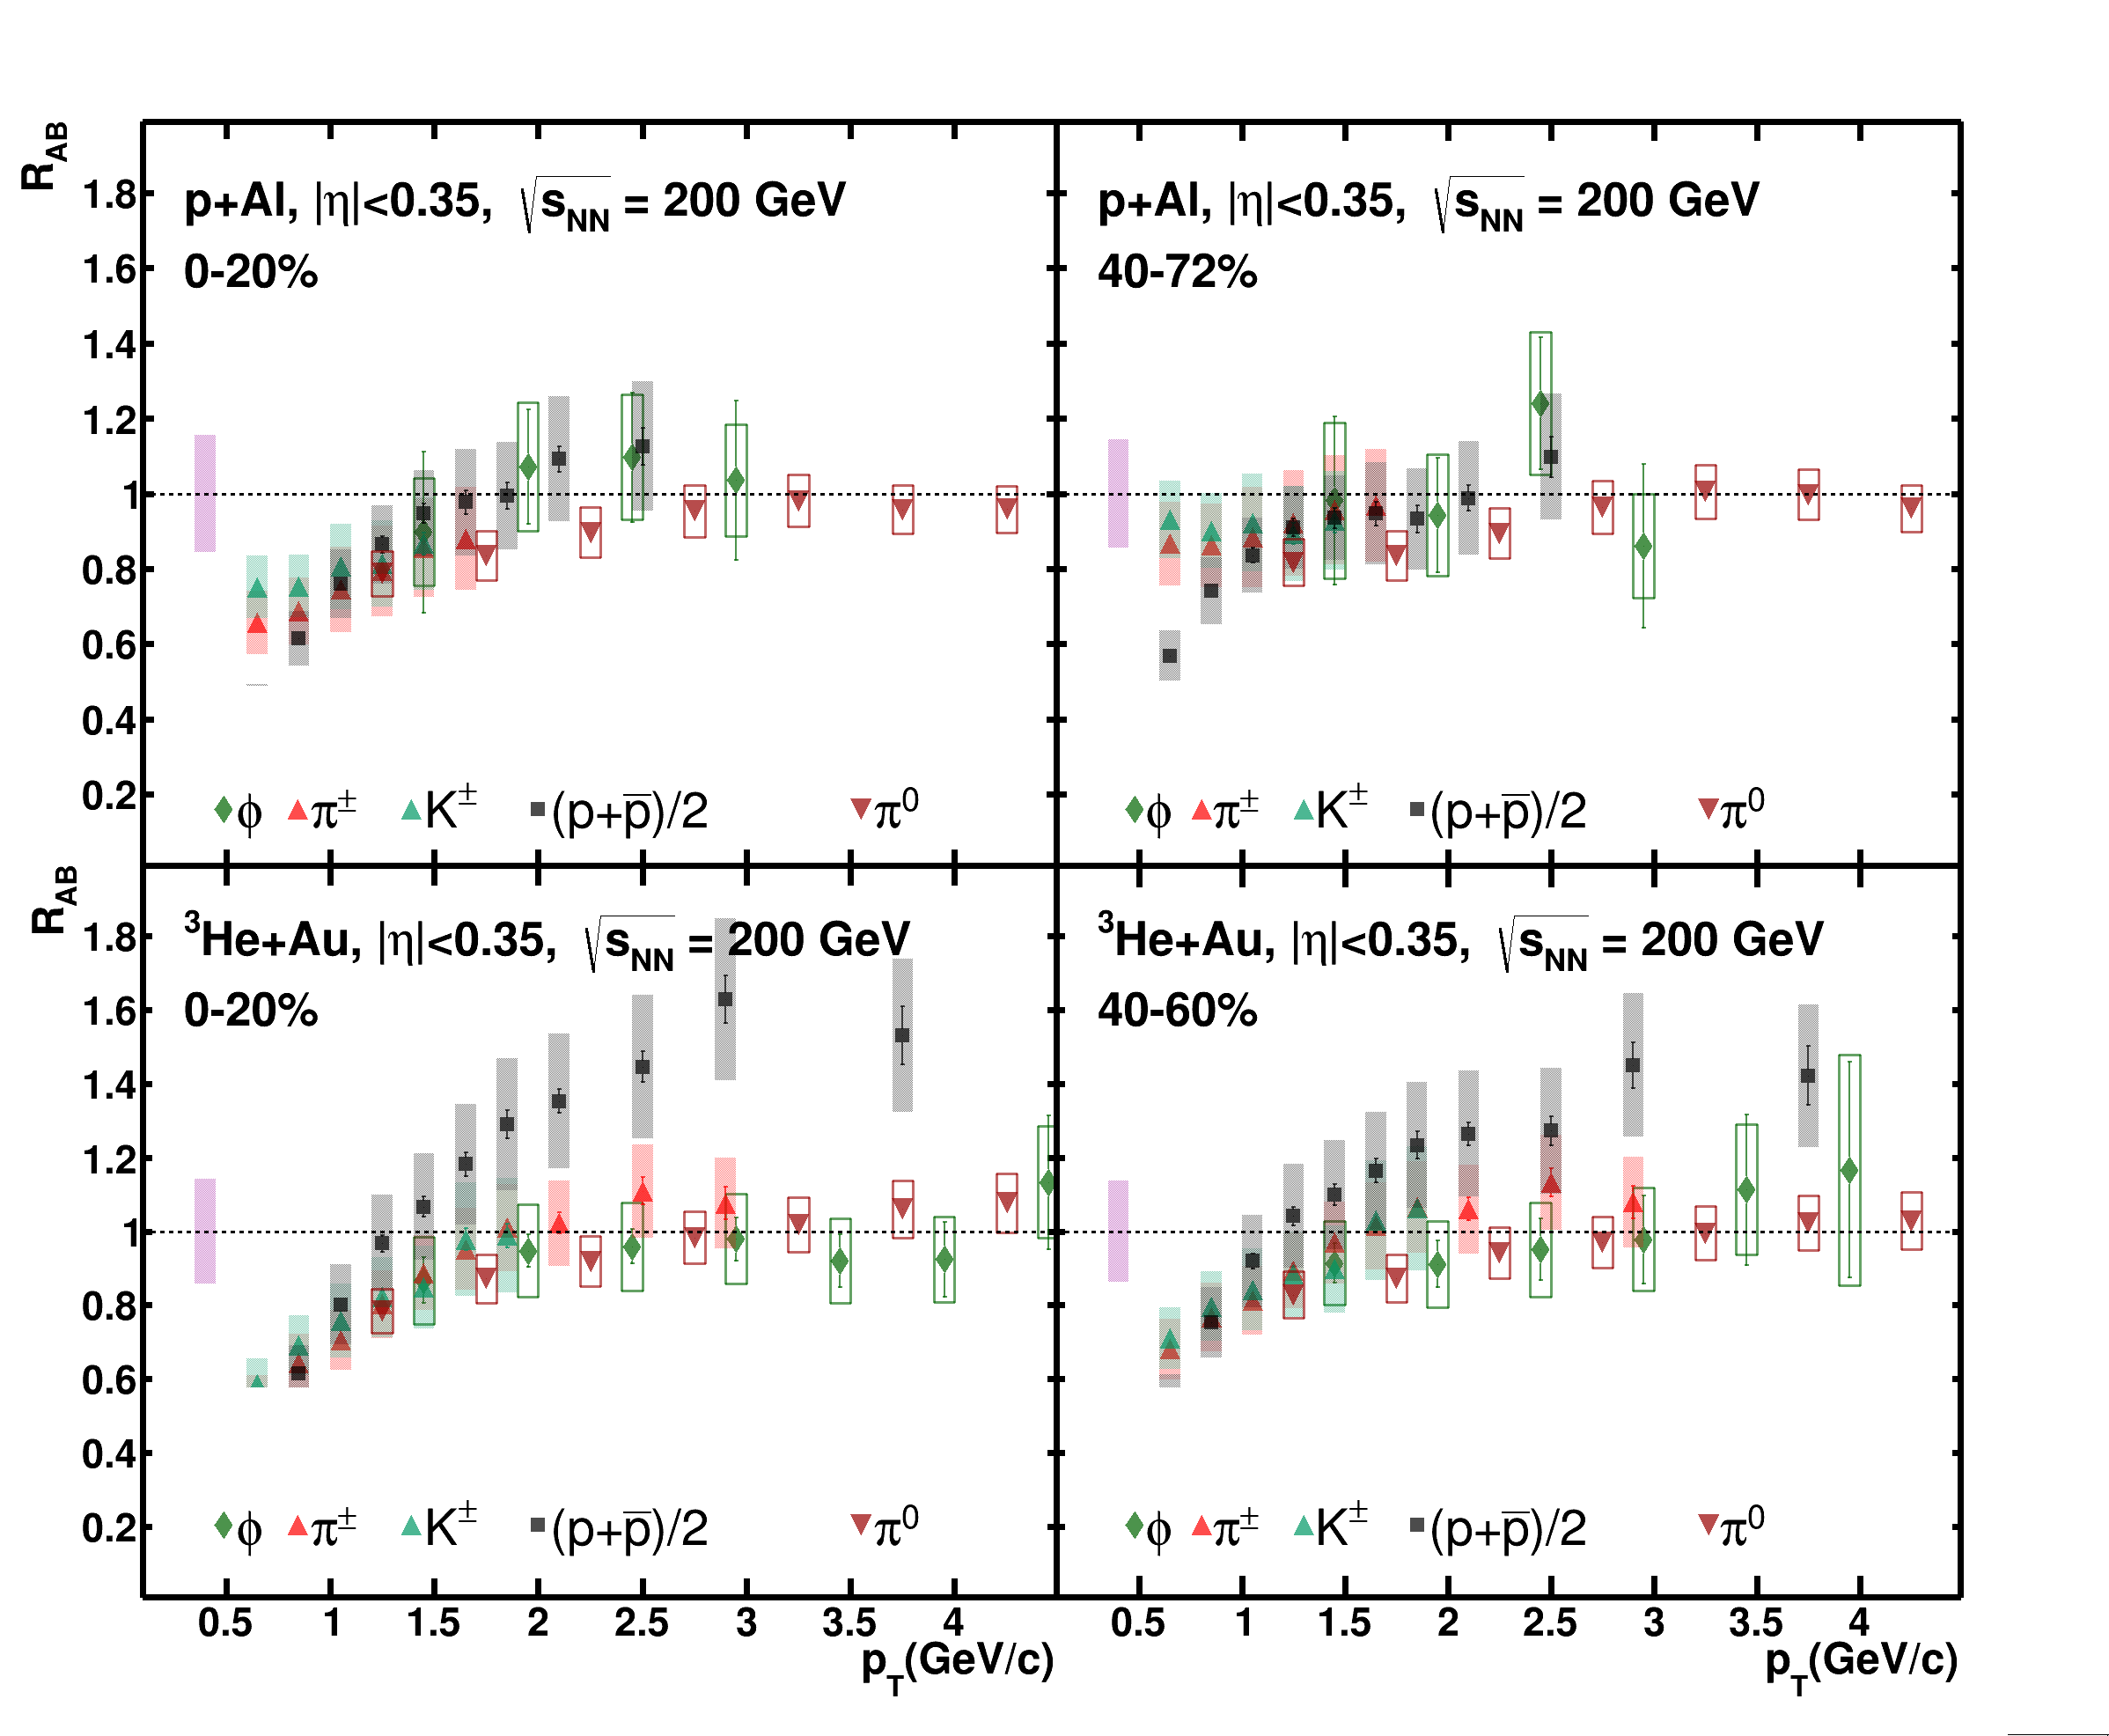
\includegraphics [width=0.7\linewidth]{Results/DrawMesons_small.png}
	\caption{Значения факторов ядерной модификации ($R_{AB}$), измеренные для легких адронов(\pipm, \Kpm, \prots, $\pi^{0}$, $\phi$) в центральных и периферических столкновениях \pal \ и \heau.} 
	\label{img:synops_DrawMesonsSmall}
\end{figure}

\begin{figure}[] 
	\centerfloat
	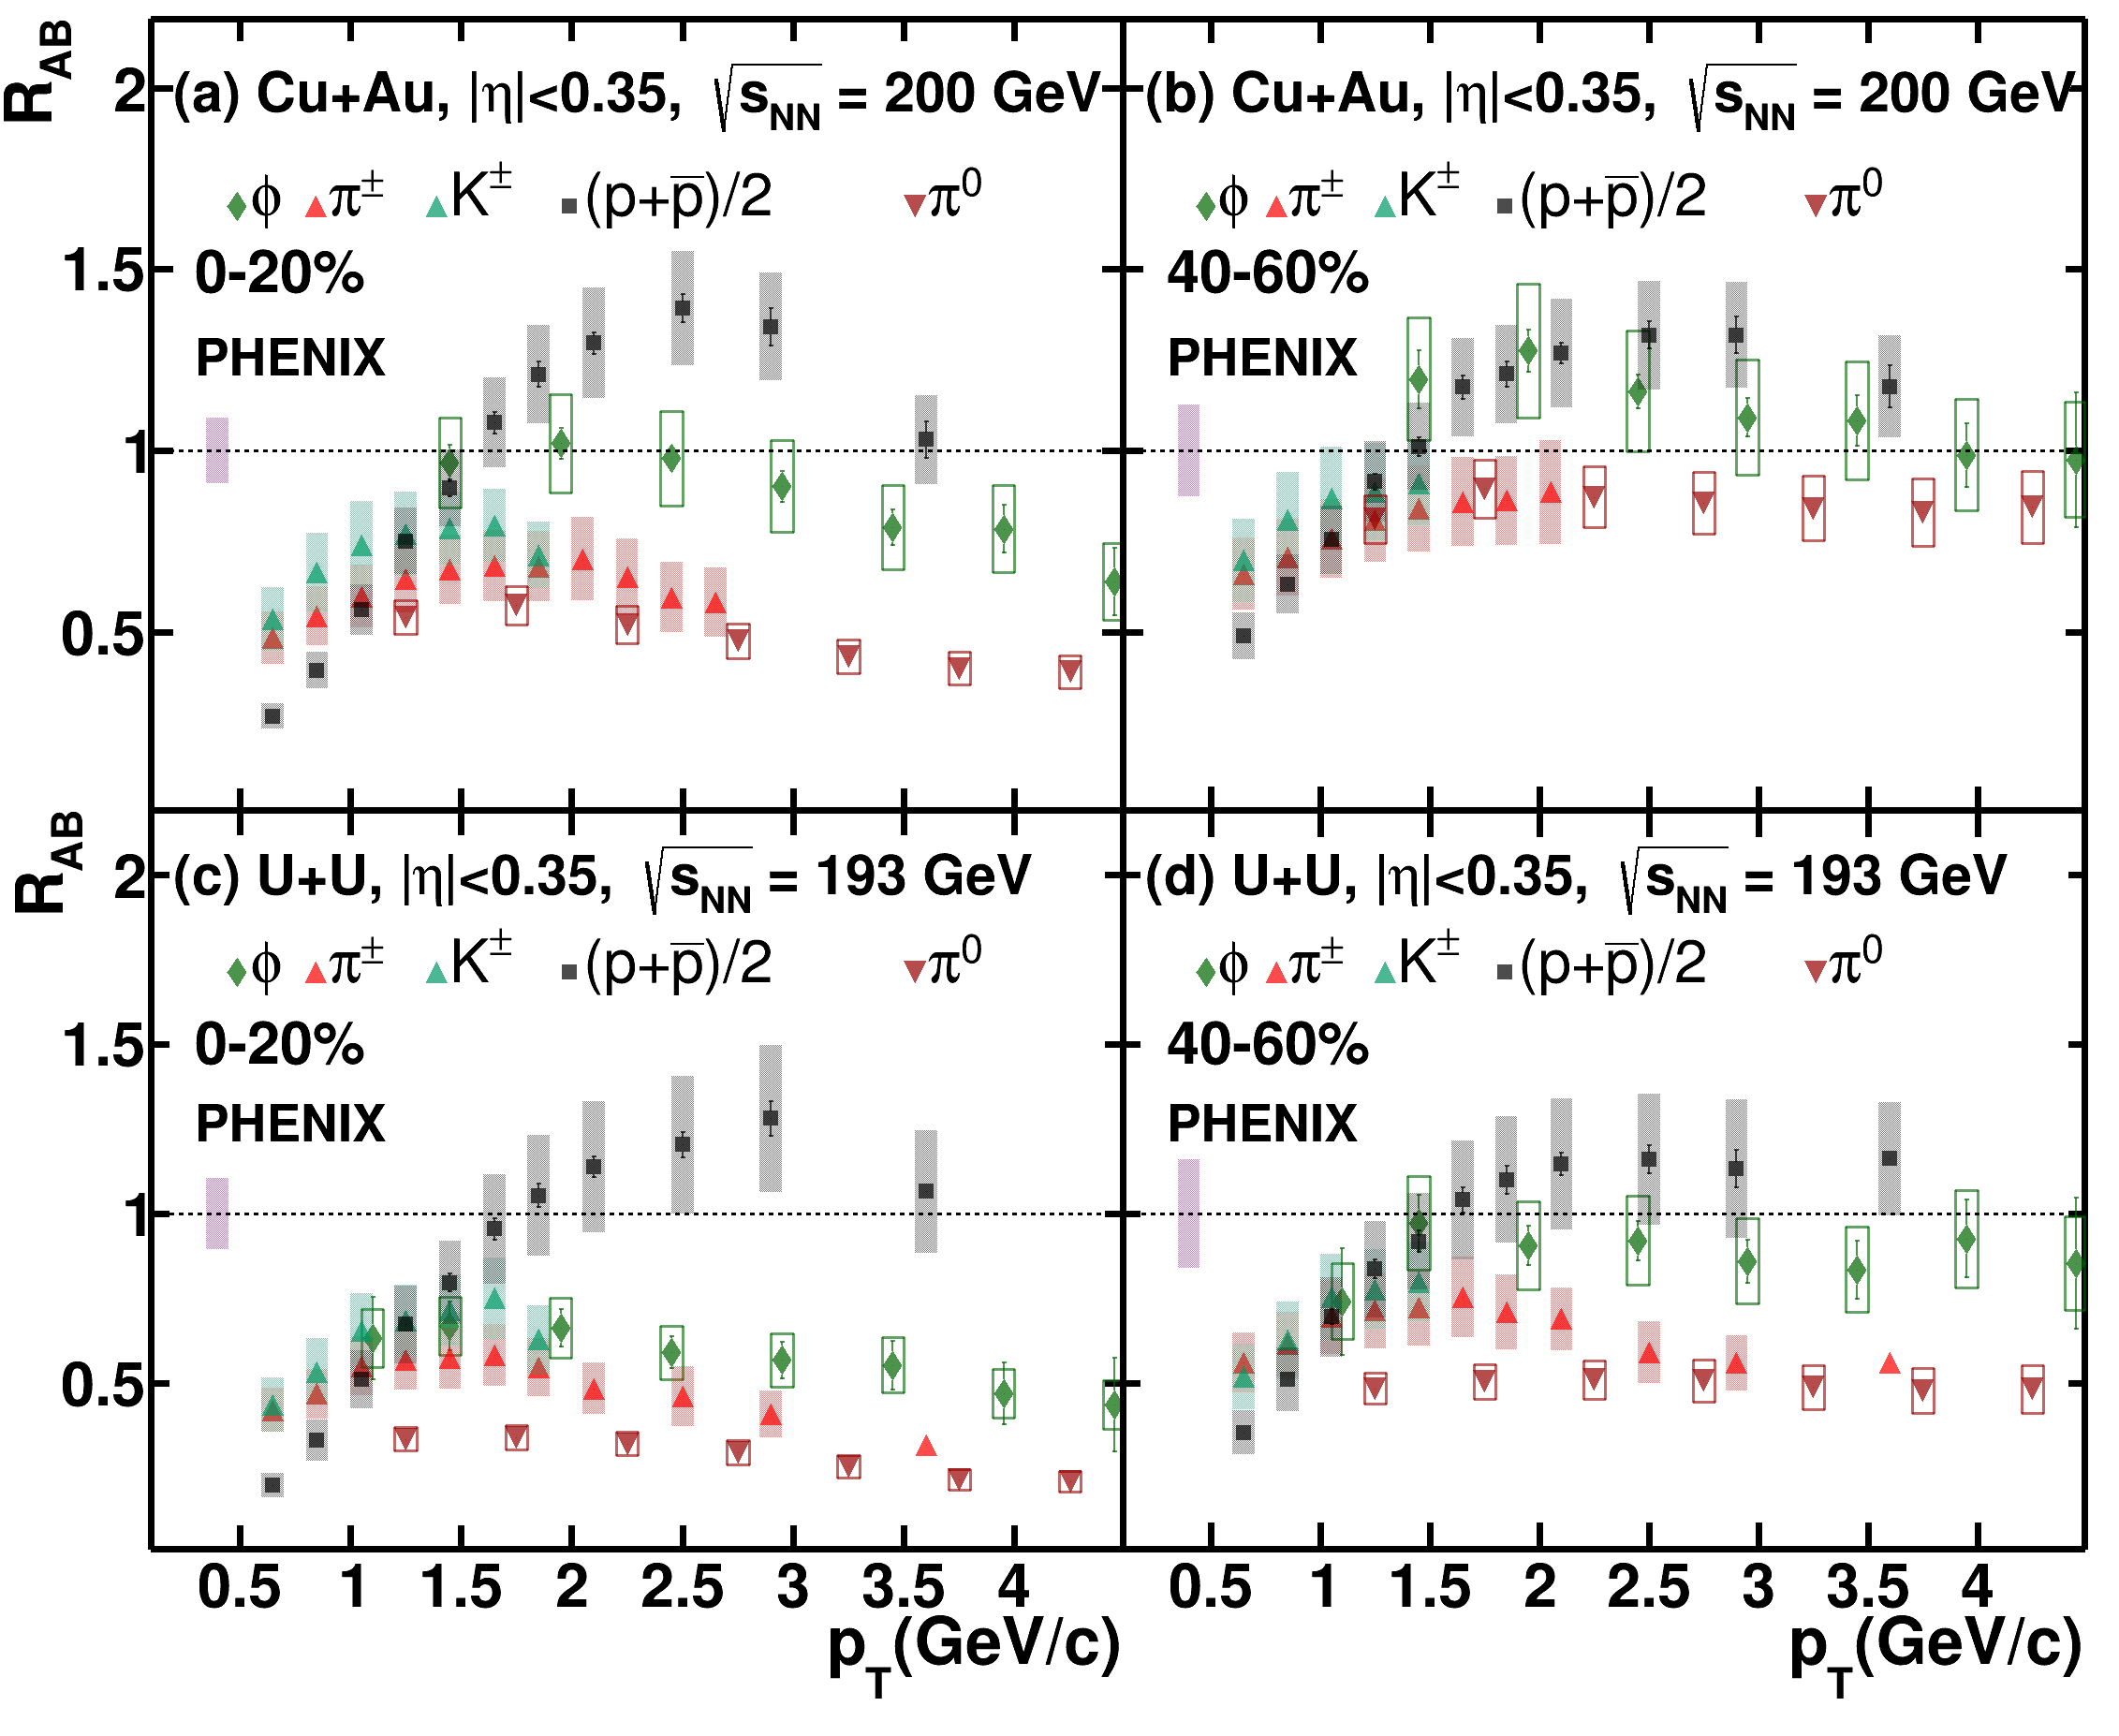
\includegraphics [width=0.7\linewidth]{Results/DrawMesons_large.png}
	\caption{Значения факторов ядерной модификации ($R_{AB}$), измеренные для легких адронов(\pipm, \Kpm, \prots, $\pi^{0}$, $\phi$) в центральных и периферических столкновениях Cu+Au и U+U.} 
	\label{img:synops_DrawMesonsLarge}
\end{figure}
\end{comment}

В центральных столкновениях \heau, Cu+Au и U+U был обнаружен эффект увеличенного выхода протонов и антипротонов, проявляющийся в увеличении значений $p/\pi$ по сравнению со значениями $p/\pi$, измеренными в $p+p$ столкновениях, а также в том, что значения $R_{AB}$, измеренные для протонов, превышают значения $R_{AB}$, измеренные для мезонов. 

%Было проведено сравнение факторов ядерной модификации, измеренных для различных легких адронов -- \pipm, \Kpm, \prots, $\pi^{0}$, $\phi$ (рис. \ref{img:synops_DrawMesonsSmall}, \ref{img:synops_DrawMesonsLarge}).

\underline{\textbf{Пятая глава}} основной части посвящена физической интерпретации полученных результатов в рамках модели коллективного теплового расширения системы частиц, а также путем сравнения с теоретическими предсказаниями моделей PYTHIA8/ANGANTYR, реализующей фрагментационную модель адронизации, и AMPT в версии с плавлением струн, учитывающей возможность адронизации путем рекомбинации кварков.

Путем построения и анализа инвариантных спектров рождения идентифицированных заряженных адронов по поперечной массе ($m_T = \sqrt{p_T^2 +m_h^2}$) особенности рождения \pipm, \Kpm, \prot, \aprot \ были интерпретированны в рамках модели радиально расширяющейся термализованной системы. Согласно данной модели, кинетическая энергия частиц складывается из энергии их теплового движения $T_0$ и энергии, приобретаемой частицами за счет радиального расширения системы ($m_h\left< u_t\right>$). Параметры $T_0$ и \ut \  интерпретируются как температура <<вымораживания>> системы и средняя скорость коллективного движения частиц. Параметры $T_{0}$ и \ut \ были вычисленны в \pal, \heau, Cu+Au и U+U столкновениях при различных значениях \Npart. 
Полученные зависимости $T_{0}(N_{part})$ и \ut(\Npart) приведены на Рисунке \ref{fig:synops_T0ut}. Величина $T_{0}\approx170$ МэВ и является постоянной относительно значений \Npart, в то время как величины \ut \ увеличиваются с увеличением значений \Npart.

\begin{figure}[ht]
	\centerfloat{
		\hfill
		\subcaptionbox{ }{%
			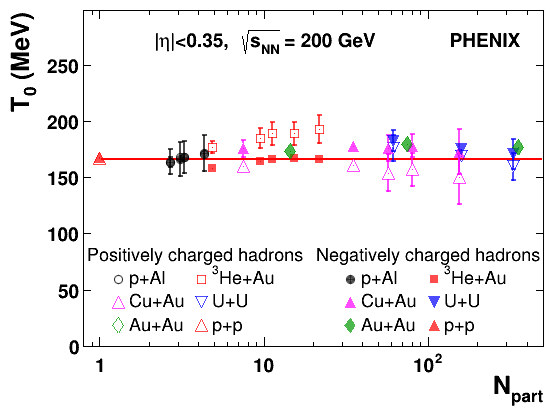
\includegraphics[width=0.45\linewidth]{Results/T0_Npart.png}}
		\hfill
		\subcaptionbox{ }{%
			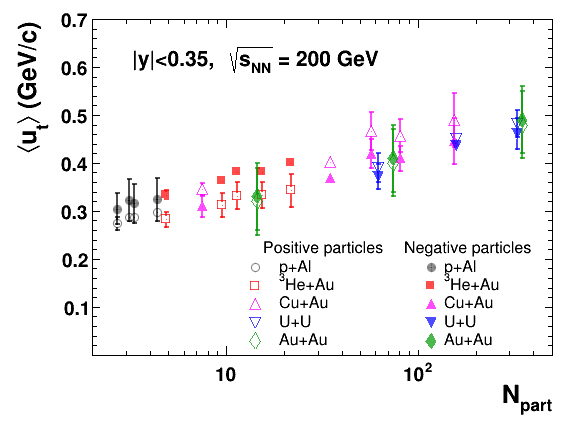
\includegraphics[width=0.45\linewidth]{Results/ut_Npart.png}}
		\hfill
	}
	\caption{Зависимость а) температуры вымораживания $T_0$ и  б) скорости поперечного потока $u_T$ от количество нуклонов участников \Npart.}\label{fig:synops_T0ut}
\end{figure}
Для более глубокого анализа особенностей рождения идентифицированных заряженных адронов было проведено сравнение измеренных значений отношений  \pim/\pip, \Km/\Kp, \prot/\aprot, \prot/\pip, \aprot/\pim, \Kp/\pip, \Km/\pim \ с предсказаниями модели PYTHIA8/ANGANTYR \cite{pythia}, реализующей фрагментационную модель адронизации, и модели AMPT в версии с плавлением струн (AMPTsm)\cite{AMPT}, учитывающей возможность адронизации путем рекомбинации кварков. 
%Для более глубокого анализа полученных экспериментальных данных, было осуществлено моделирование \pal, \heau, Cu+Au столкновений при \sqsn \= 200 ГэВ и U+U столкновений при \sqsn \= 193 ГэВ с помощью программных пакетов PYTHA8.3/ANGANTYR \cite{pythia} и AMPT \cite{AMPT}. 
Результаты представлены на Рисунках \ref{img:synops_Ratio_LargeP2PI_sym}-\ref{img:synops_Ratio_SmallK2PI_sym}.
На основе сравнения эеспериментальных результатов и предсказаний моделей мделаны следующие выводы:

\begin{enumerate}
	\item Предсказания значений $p/\pi$ моделью PYTHIA8.3/ANGANTYR, использующей фрагменационный механизм адронизации, совпадают в пределах погрешностей с экспериментальными результатами, полученными в $p$+$p$ столкновениях. 
	\item Модель AMPTsm позволяет качественно (но не количественно) описать рост значений $p/\pi$, наблюдаемый в эксперименте в центральных \heau, Cu+Au и U+U столкновениях, а также зависимость этих значений от центральности. 
	\item Величины $p/\pi$, полученные с помощью модели AMPTsm, численно не совпадают с экспериментально измеренными. 
	\item В $p$+$p$, \pal, а также перефирических \heau, Cu+Au и U+U столкновениях, значения $p/\pi$, полученные с помощью моделей PYTHIA8.3/ANGANTYR и AMPT совпадают в пределах погрешностей.
	\item Предсказания величин $K/\pi$ моделью AMPTsm согласуются с экспериментальными результатами, в то время как модель PYTHIA8.3/ANGANTYR недооценивает величины $K/\pi$.
\end{enumerate}

%Согласно екомбинационной модели, $p_T$ произведенного адрона представляет собой сумму $p_T$ составляющих его кварков. Поэтому барионно-инвариантные спектры $p_T$ сдвинуты относительно мезонных спектров $p_T$ в сторону больших $p_T$, что приводит к увеличению производства барионов по сравнению с производством мезонов в промежуточной области $p_T$.
%Общее число барионов и мезонов, образующихся в процессах рекомбинации, пропорционально числу партонов внутри QGP.
%Следовательно, рост значений $p/\pi$ с увеличением центральности Cu+Au и U+U может свидетельствовать об усилении влияния рекомбинационных процессов и увеличении числа партонов в столкновении QGP. Согласие между предсказаниями модели рекомбинации и модели фрагментации в столкновениях с \Npart $\lesssim$10 может указывать на то, что объем образующегося QGP недостаточен для наблюдаемого увеличения выхода барионов.

\begin{comment}
\begin{figure}[] 
	\centerfloat
	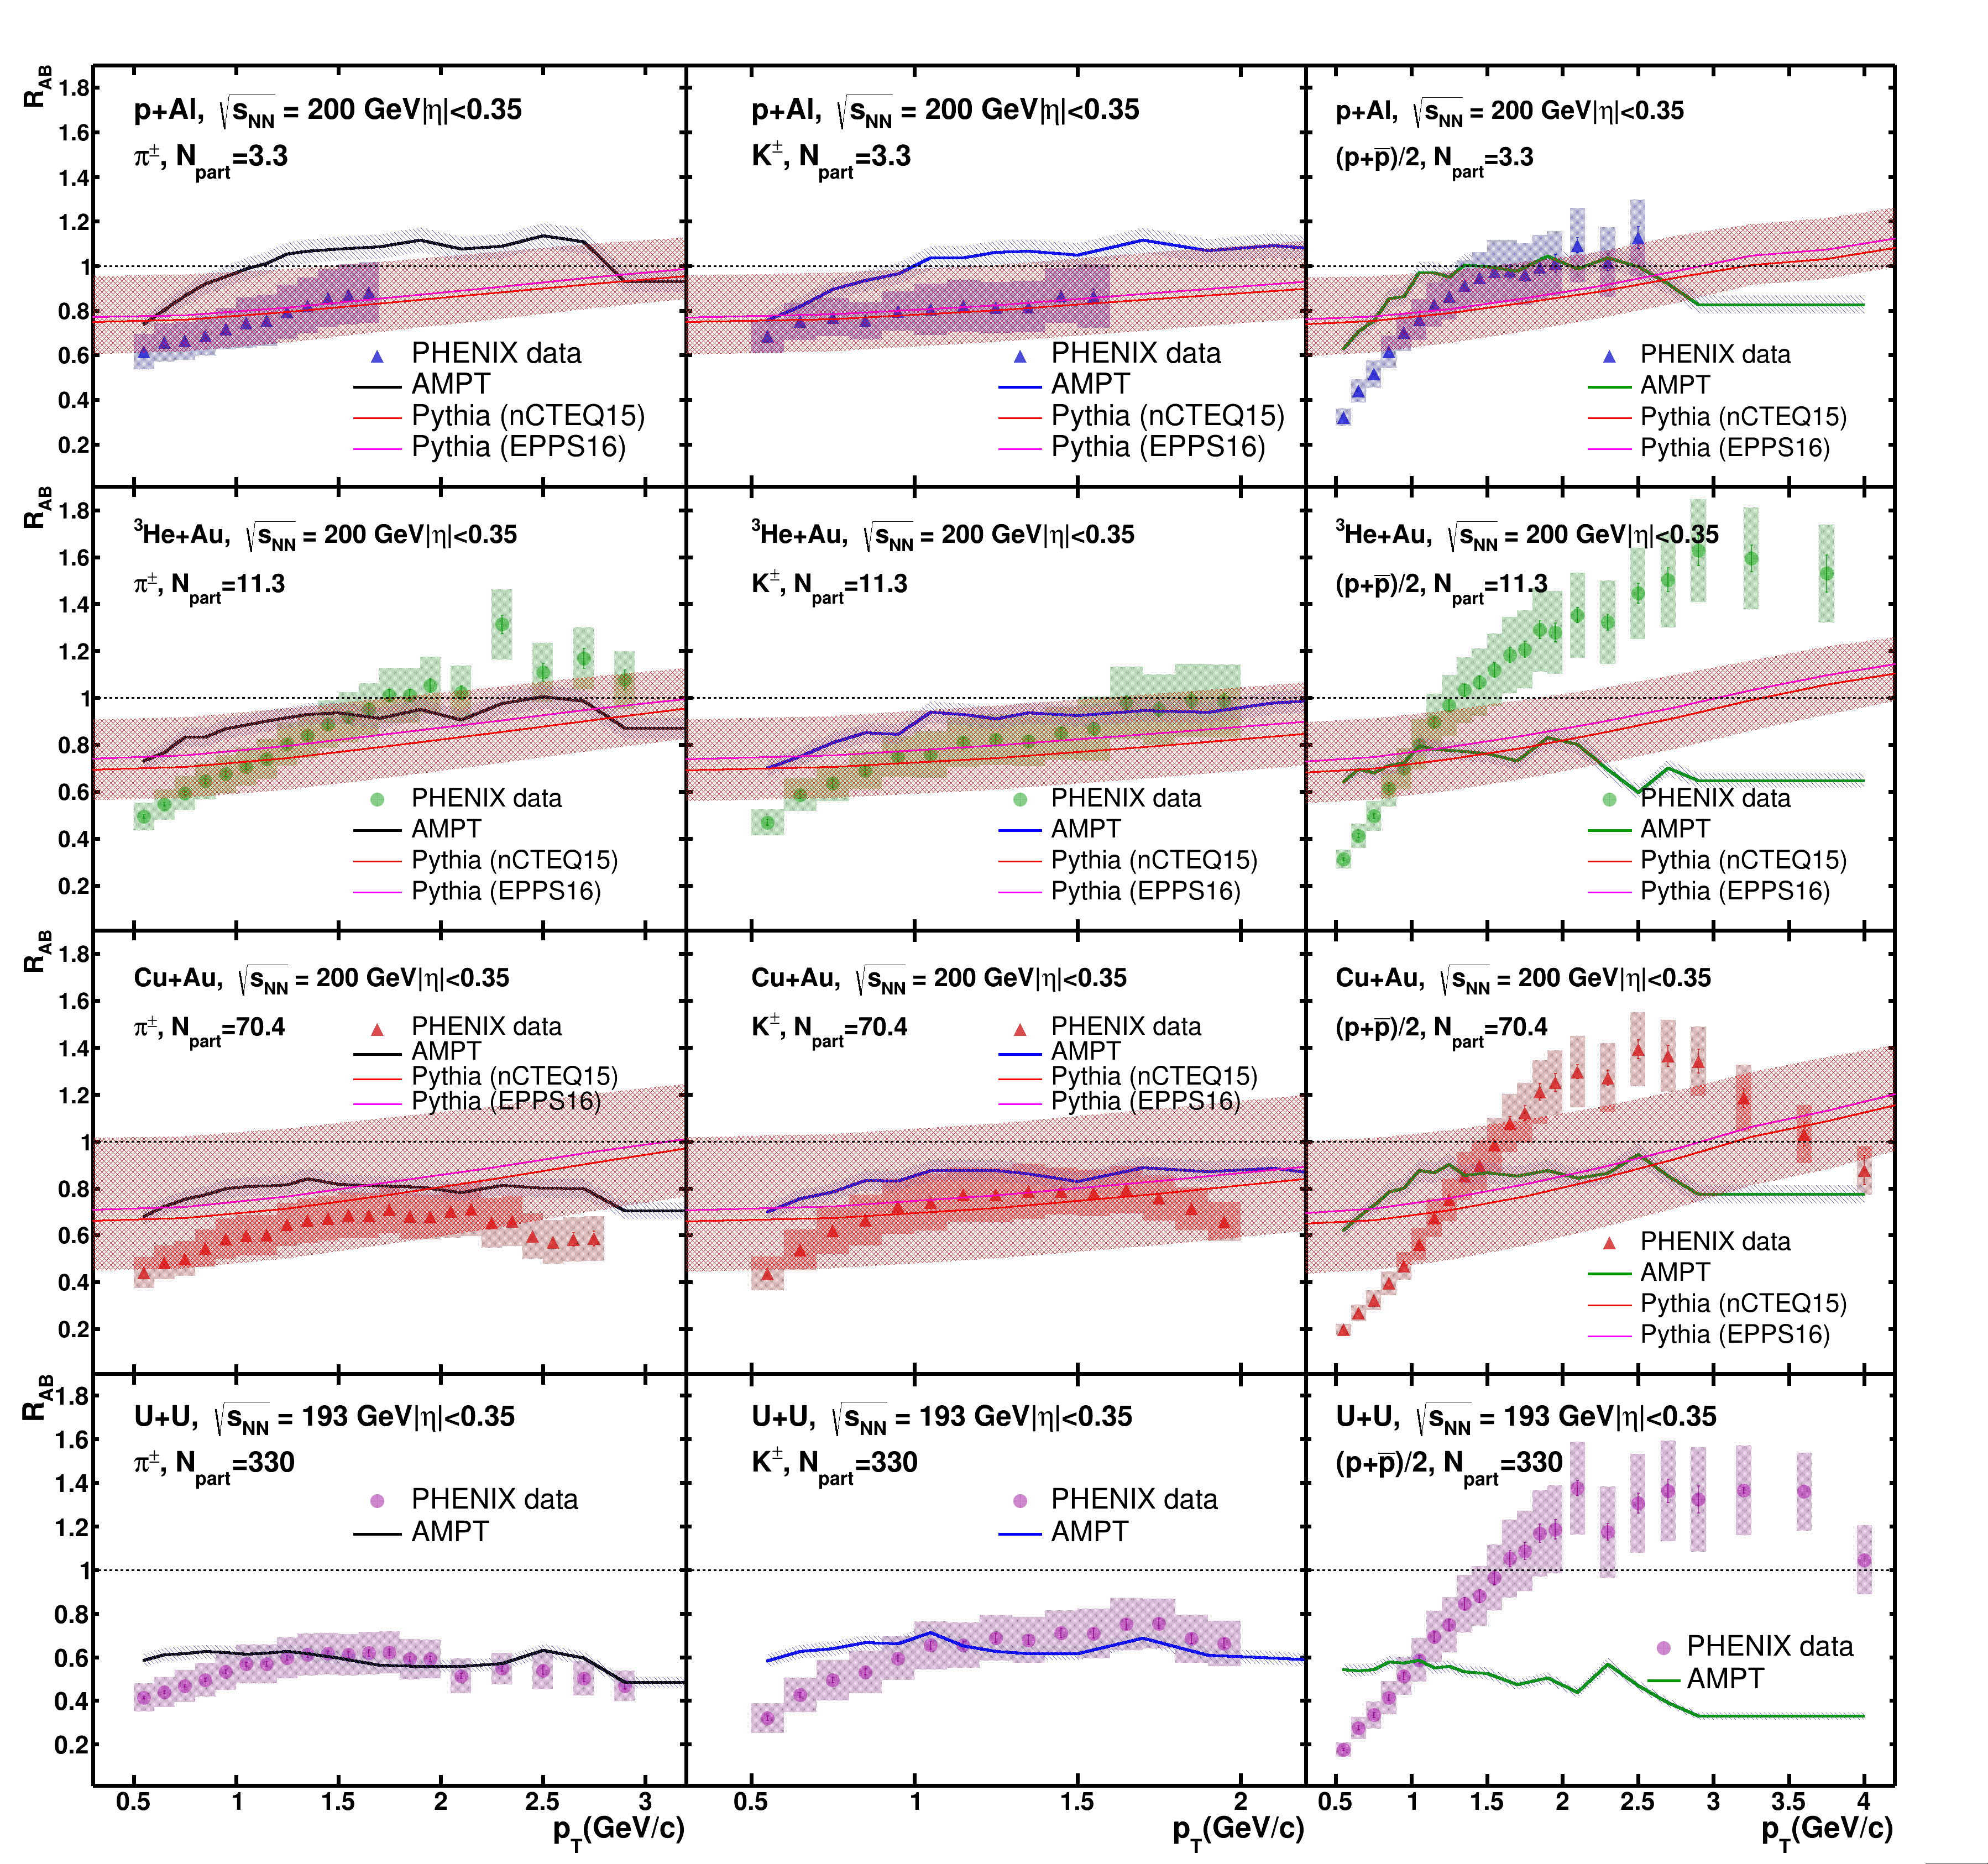
\includegraphics [width=0.8\linewidth]{Simulation/RAA_AMPT_Pythia.png}
	\caption{Инвариантные спектры по поперечному массе, измеренные для отрицательно заряженных адронов в различных центральностях p+Al, \heau, Cu+Au и U+U столкновениях.} 
	\label{img:synops_RAA_sym}
\end{figure}


\begin{figure}[] 
	\centerfloat
	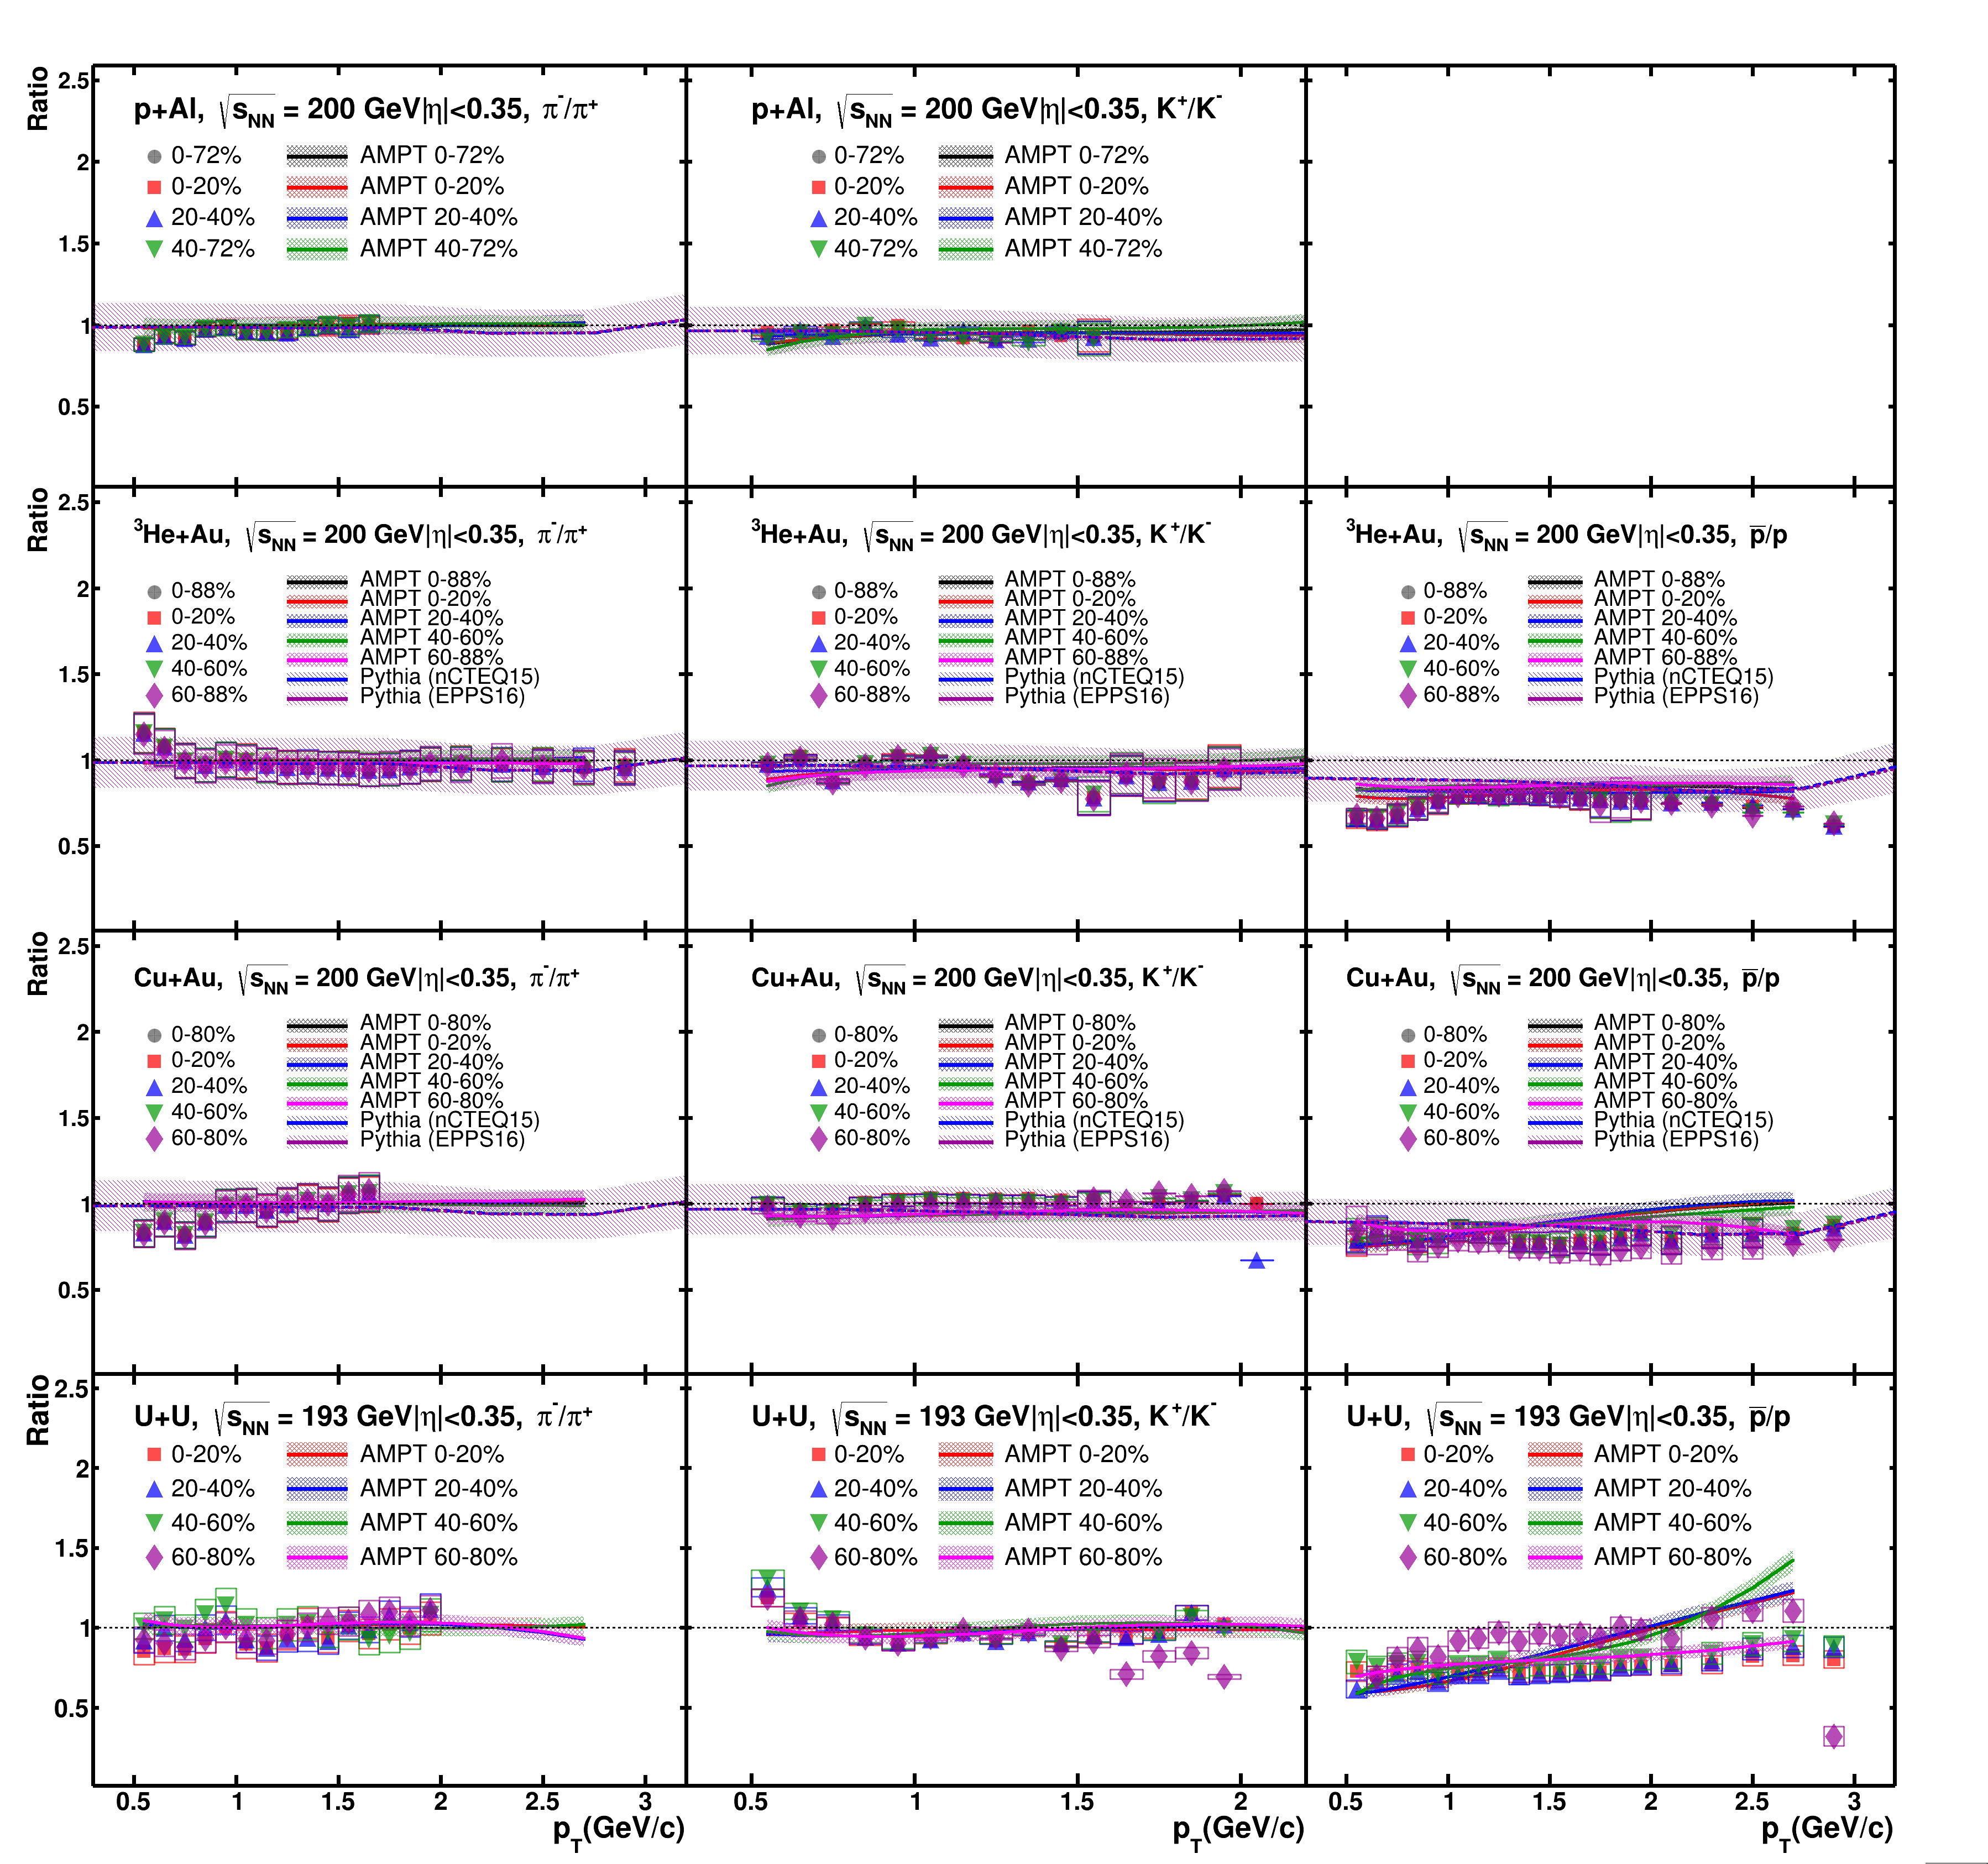
\includegraphics [width=0.6\linewidth]{Simulation/Ratio_same_AMPT_Pythia.png}
	\caption{Инвариантные спектры по поперечному массе, измеренные для отрицательно заряженных адронов в различных центральностях p+Al, \heau, Cu+Au и U+U столкновениях.} 
	\label{img:synops_Ratio_same_sym}
\end{figure}
\end{comment}

\begin{figure}[] 
	\centerfloat
	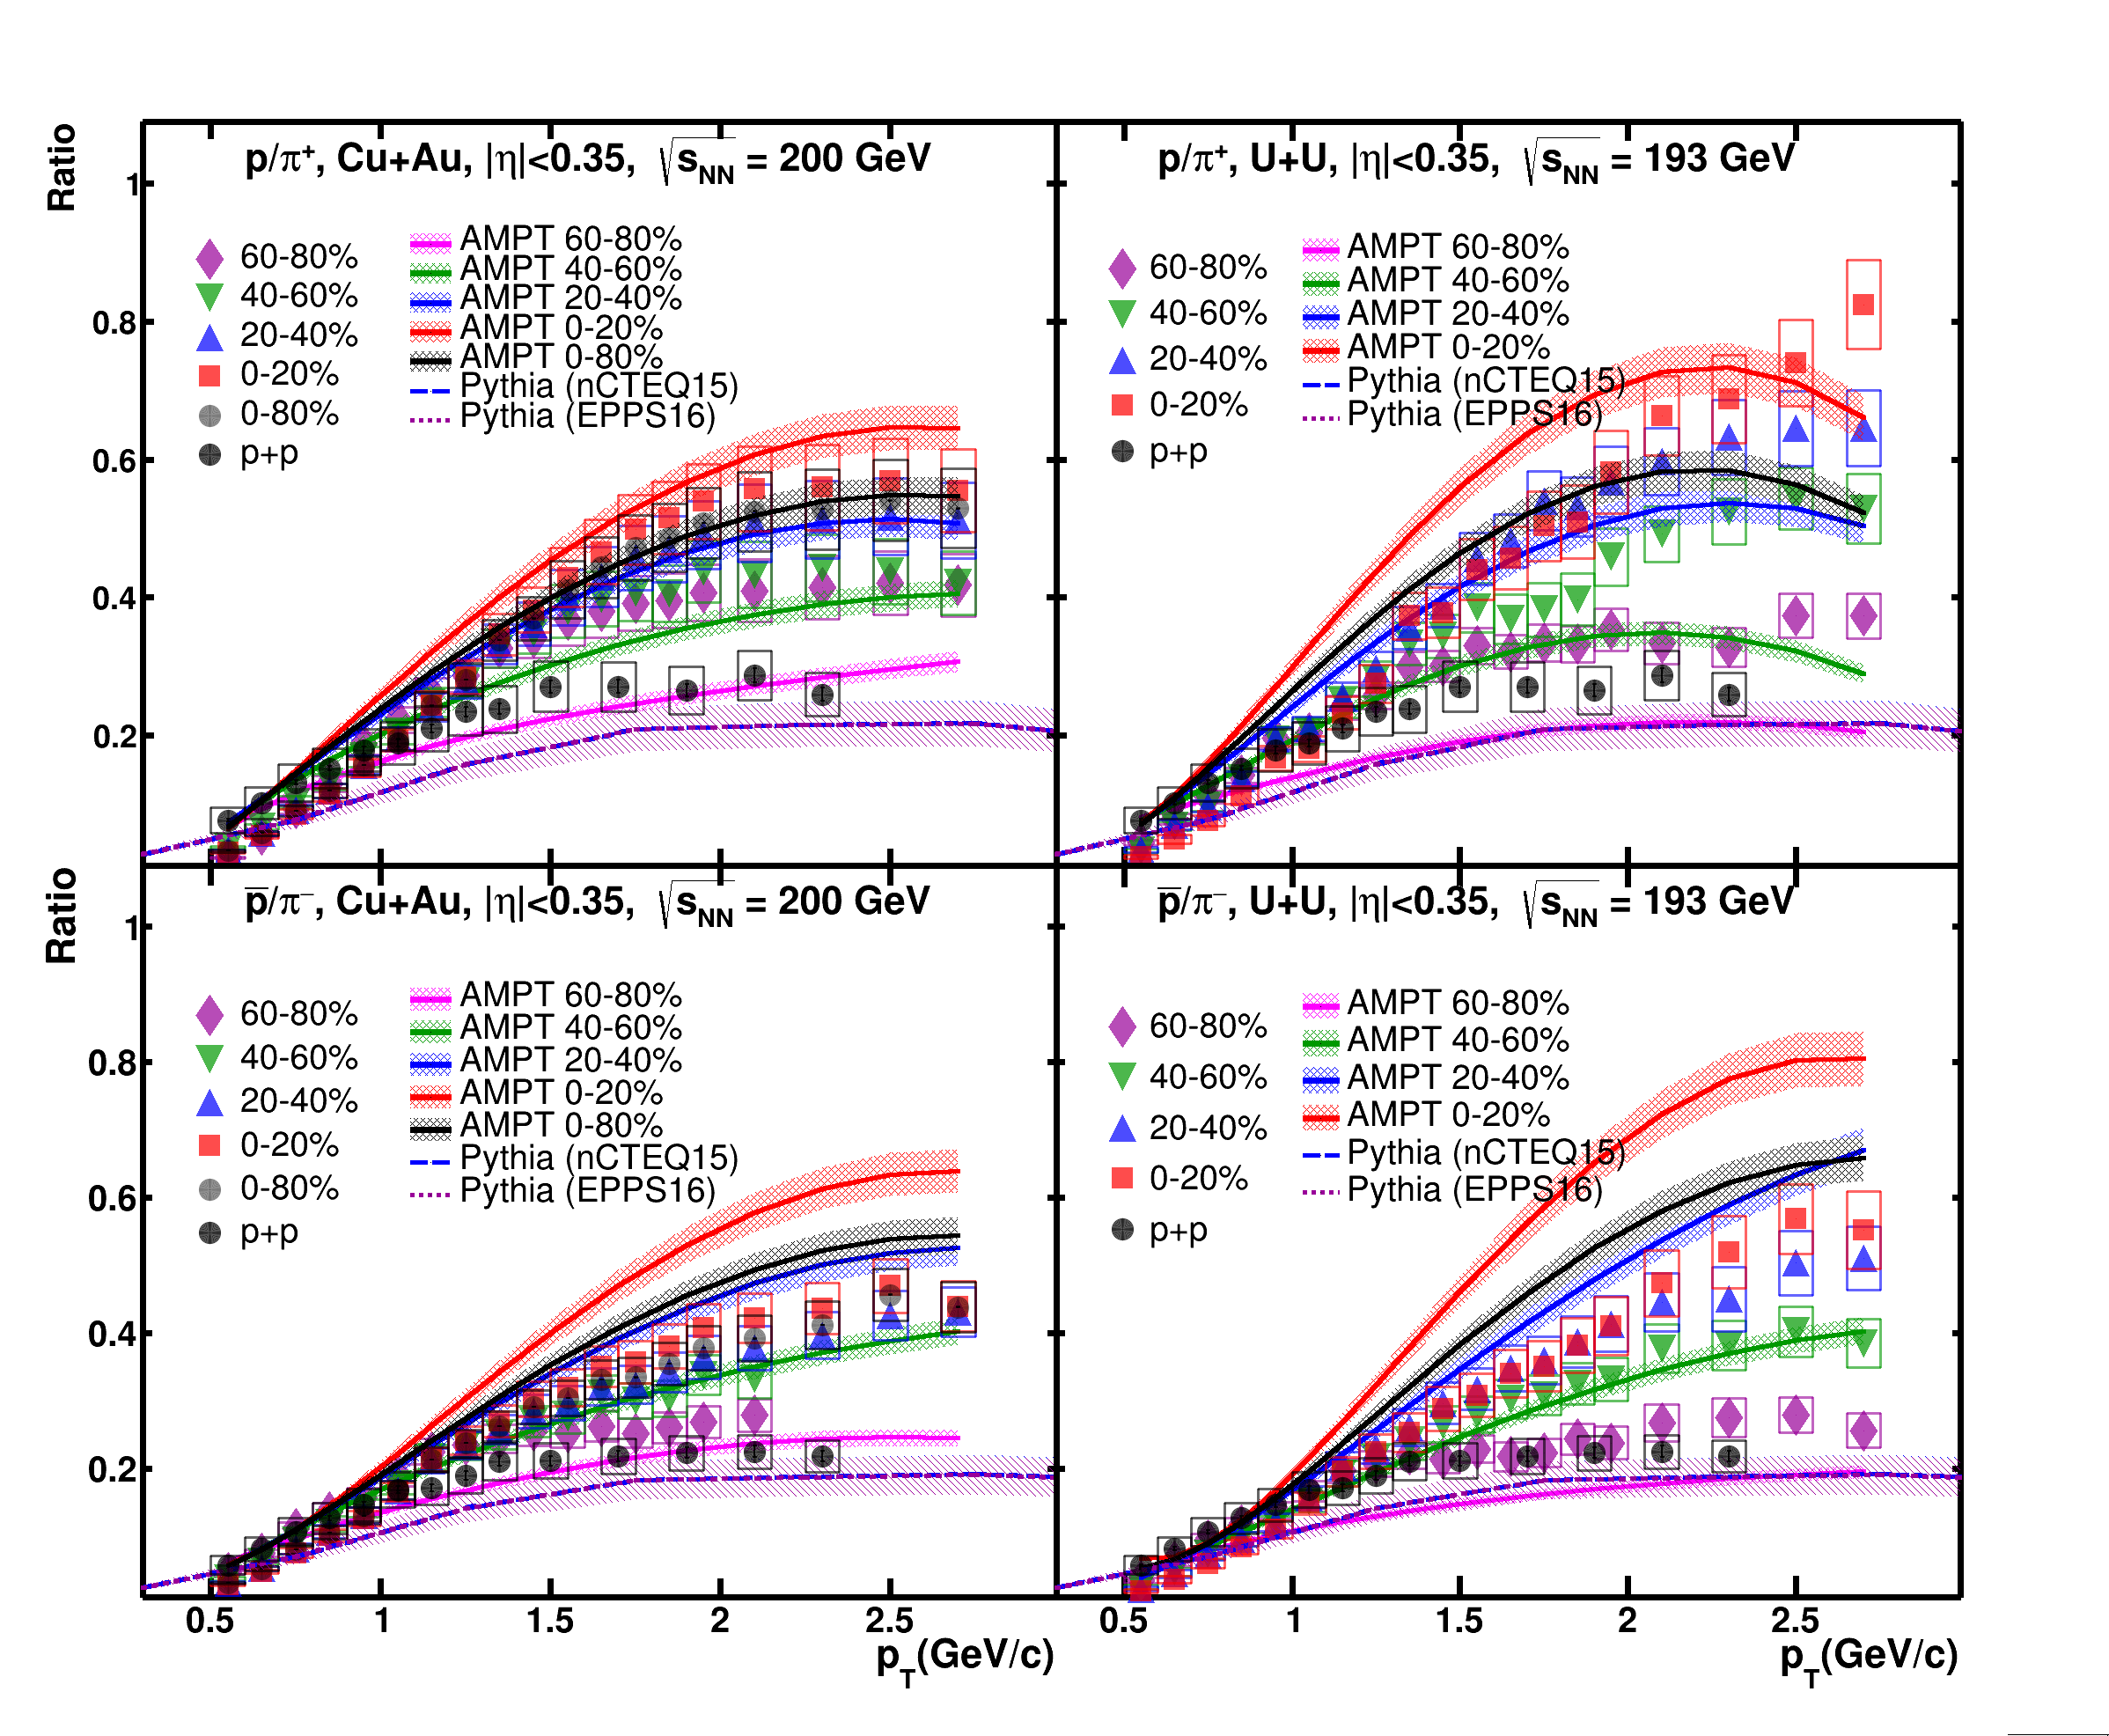
\includegraphics [width=0.7\linewidth]{Simulation/Ratios_AMPT_large_p2pi.png}
	\caption{Инвариантные спектры по поперечному массе, измеренные для отрицательно заряженных адронов в различных центральностях \pal, \heau, Cu+Au и U+U столкновениях.} 
	\label{img:synops_Ratio_LargeP2PI_sym}
\end{figure}

\begin{figure}[] 
	\centerfloat
	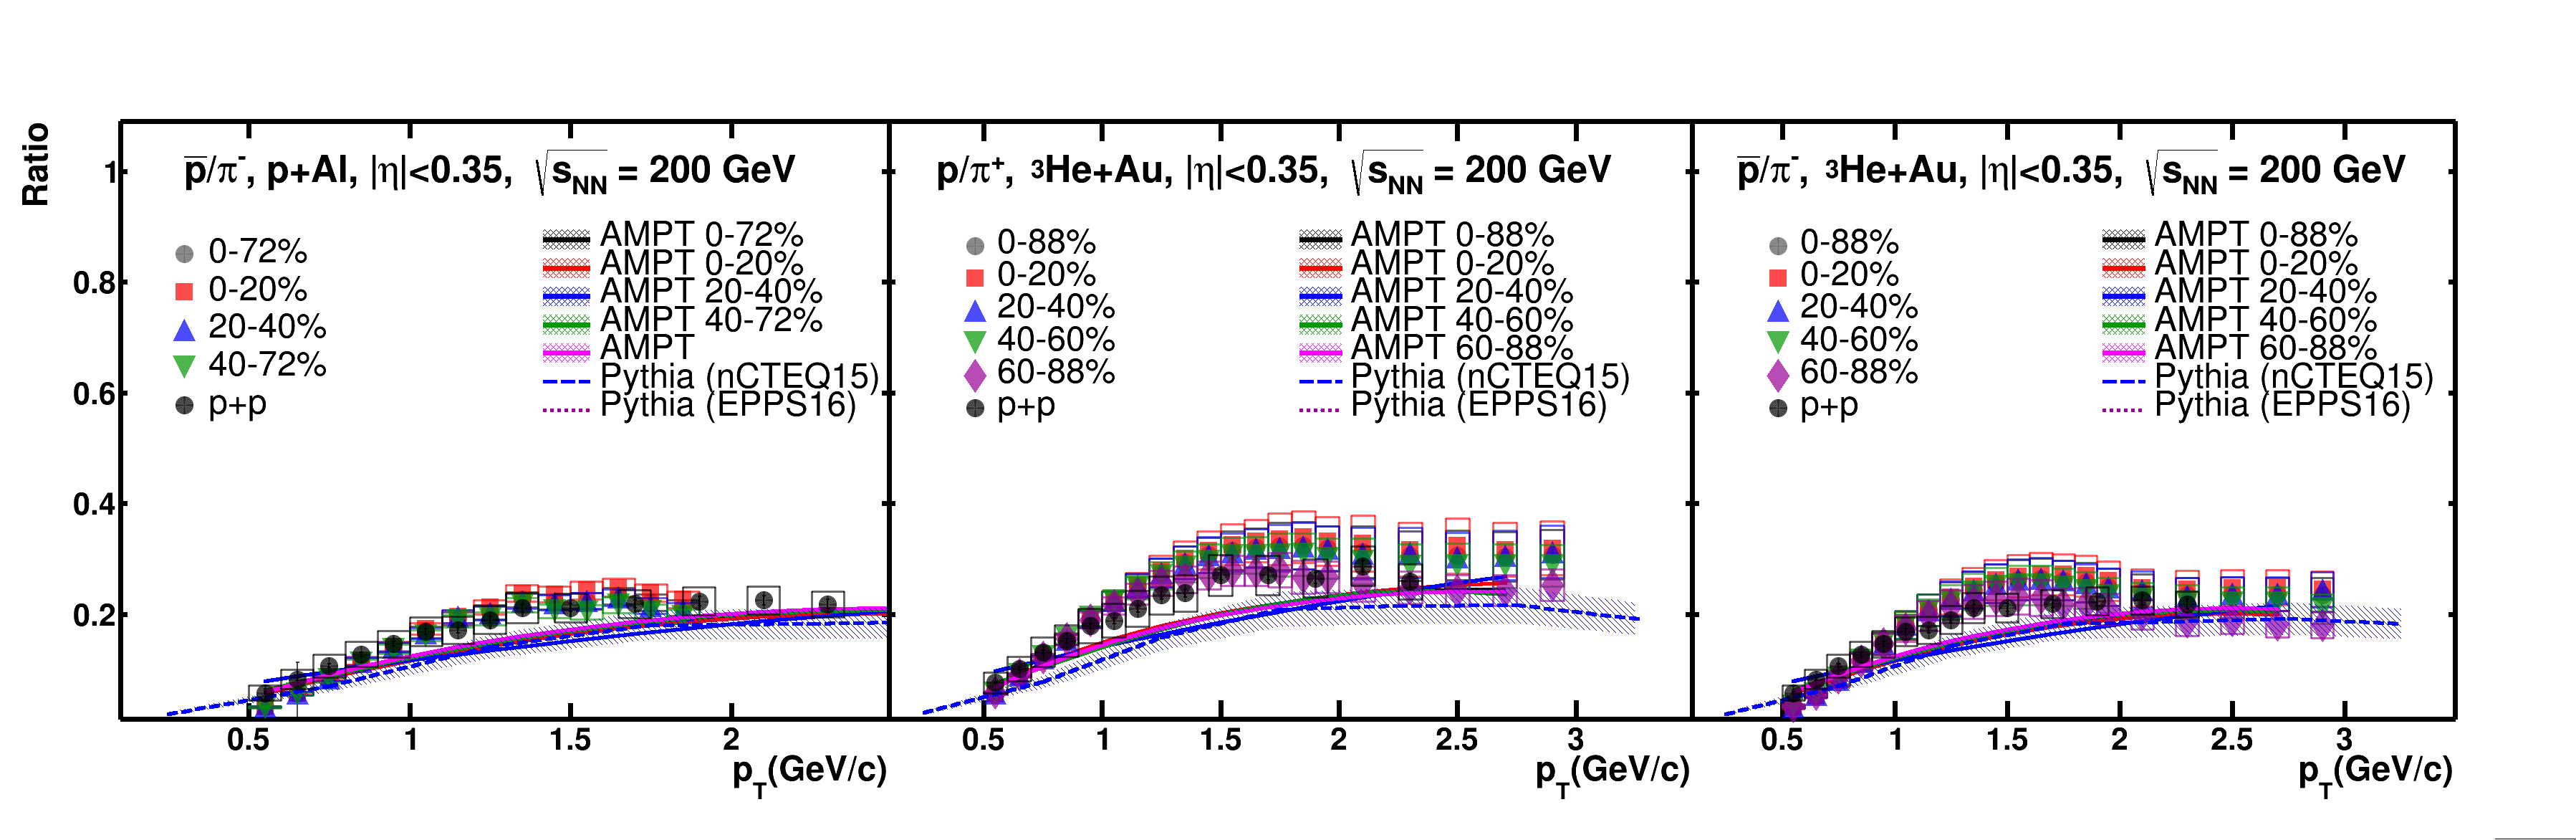
\includegraphics [width=1\linewidth]{Simulation/Ratios_AMPT_small_p2pi.png}
	\caption{Инвариантные спектры по поперечному массе, измеренные для отрицательно заряженных адронов в различных центральностях \pal, \heau, Cu+Au и U+U столкновениях.} 
	\label{img:synops_Ratio_SmallP2PI_sym}
\end{figure}

\begin{figure}[] 
	\centerfloat
	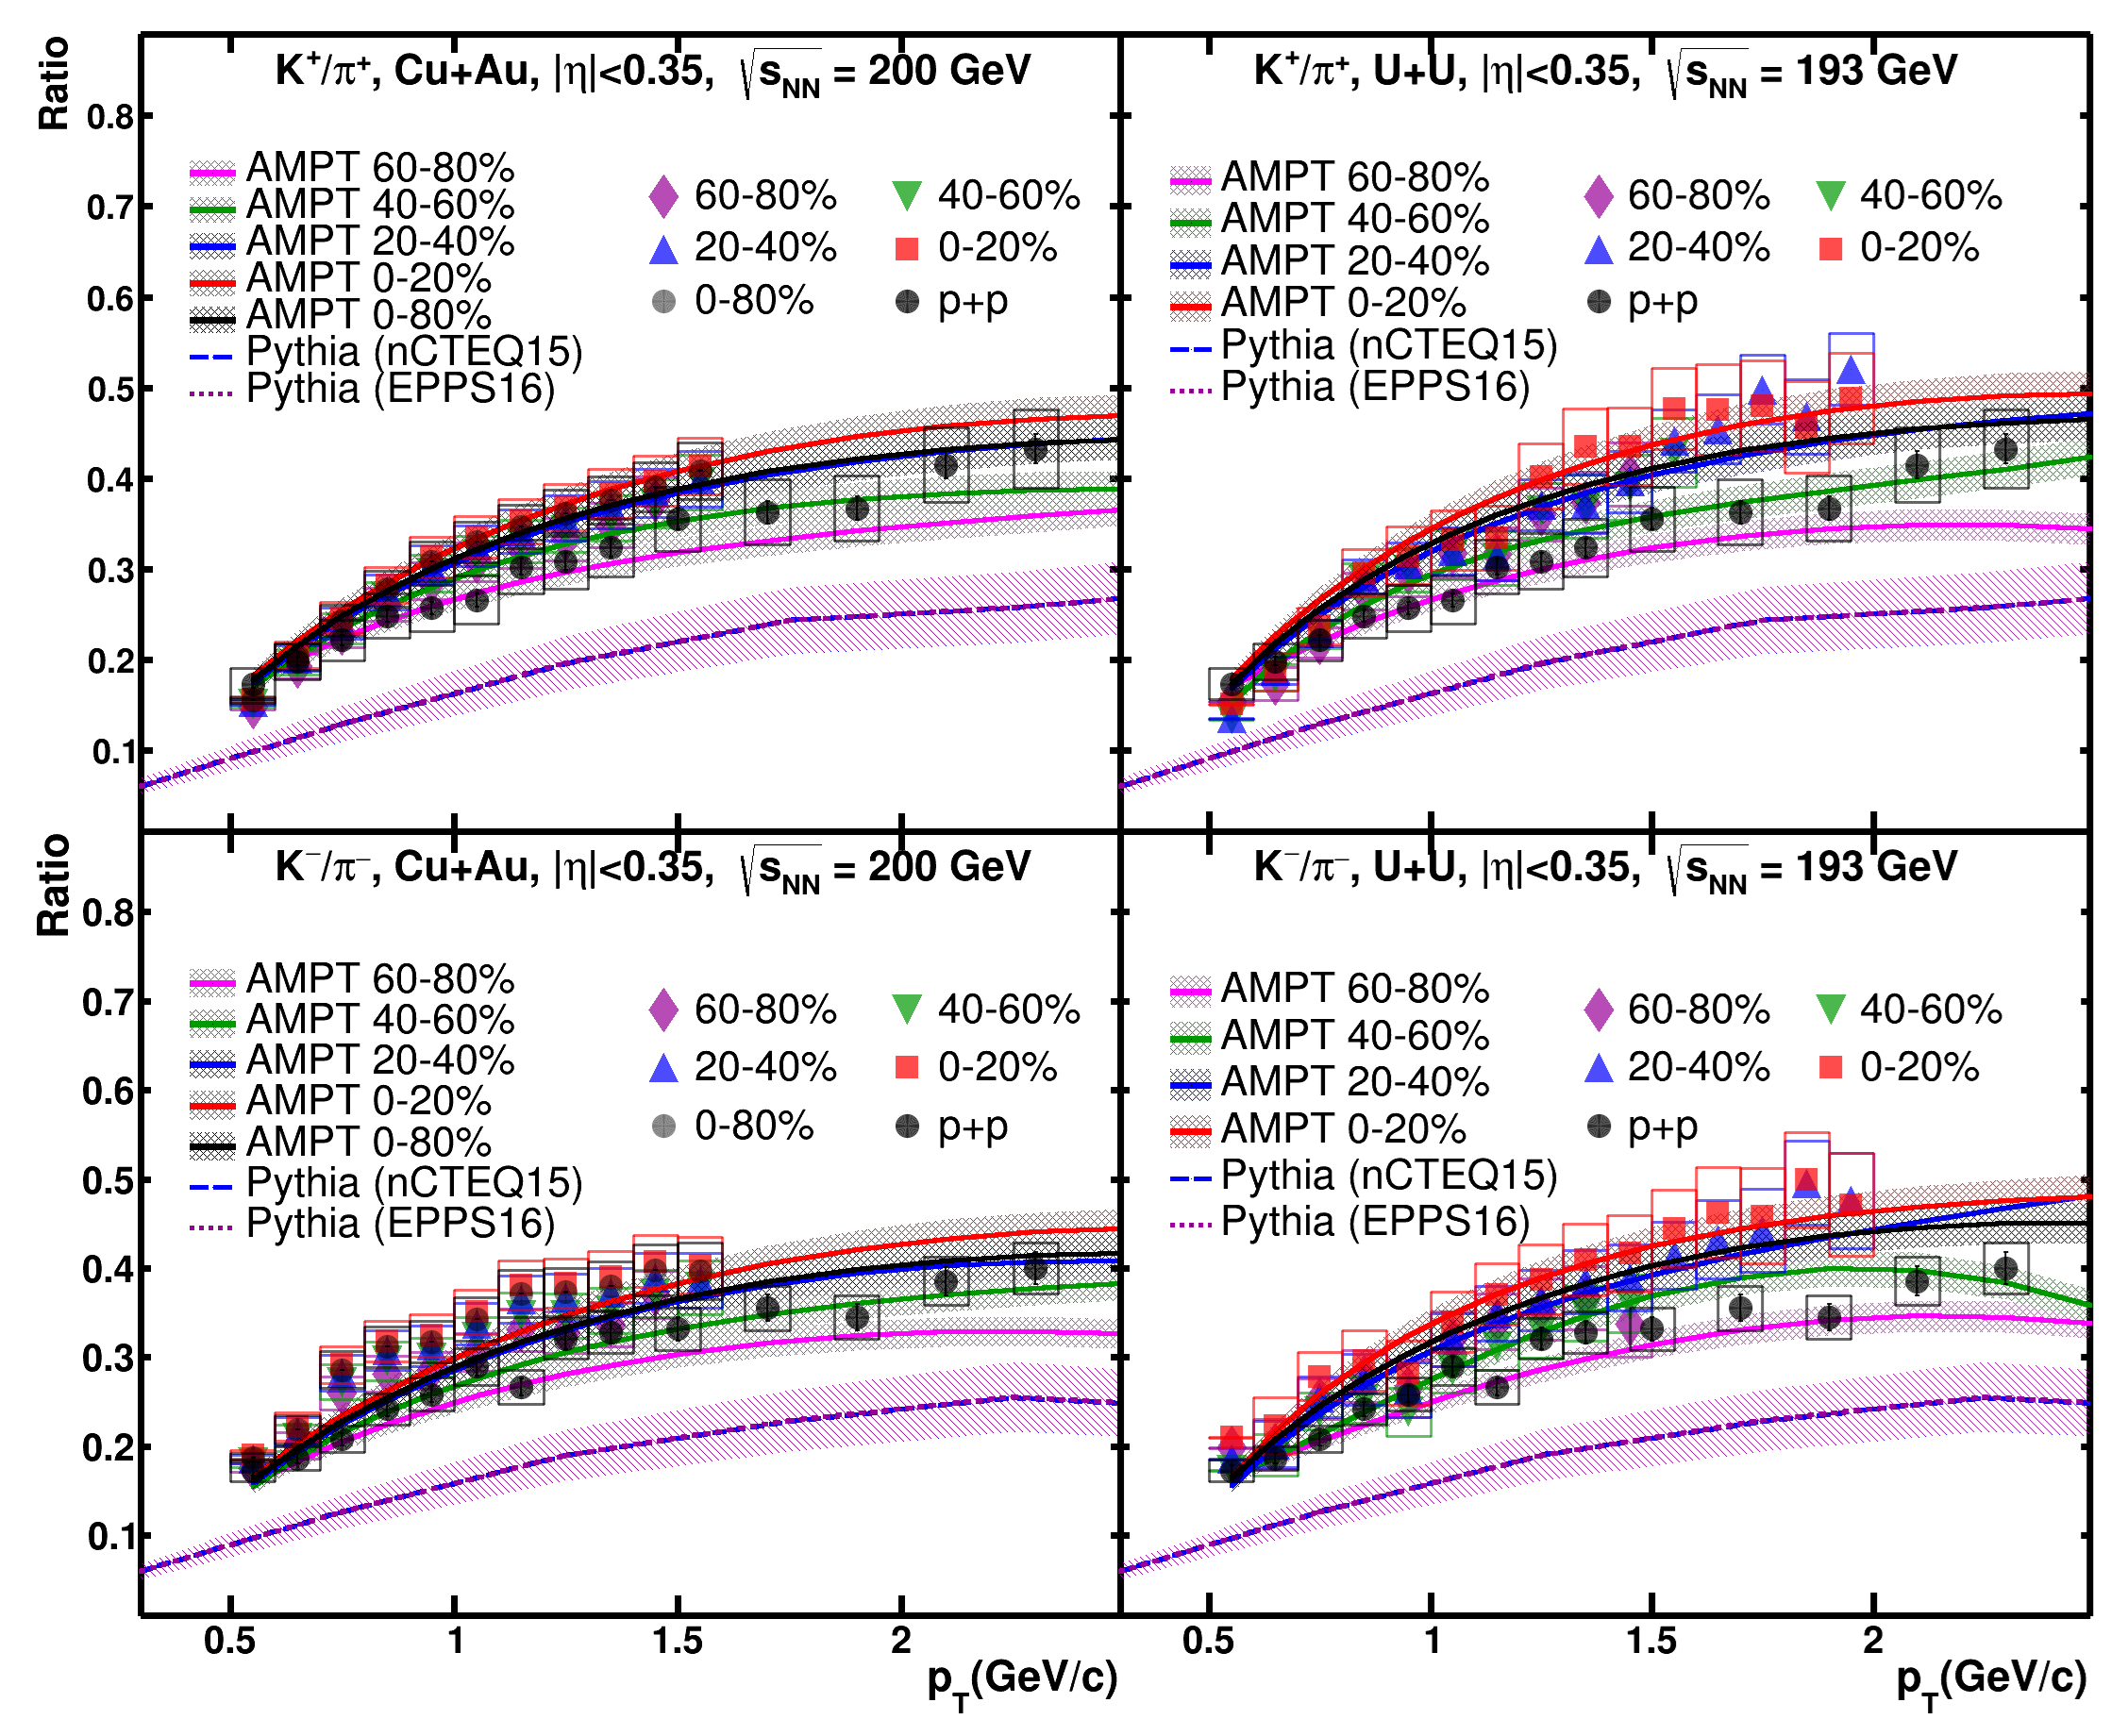
\includegraphics [width=0.7\linewidth]{Simulation/Ratios_AMPT_large_K2pi.png}
	\caption{Инвариантные спектры по поперечному массе, измеренные для отрицательно заряженных адронов в различных центральностях \pal, \heau, Cu+Au и U+U столкновениях.} 
	\label{img:synops_Ratio_LargeK2PI_sym}
\end{figure}

\begin{figure}[] 
	\centerfloat
	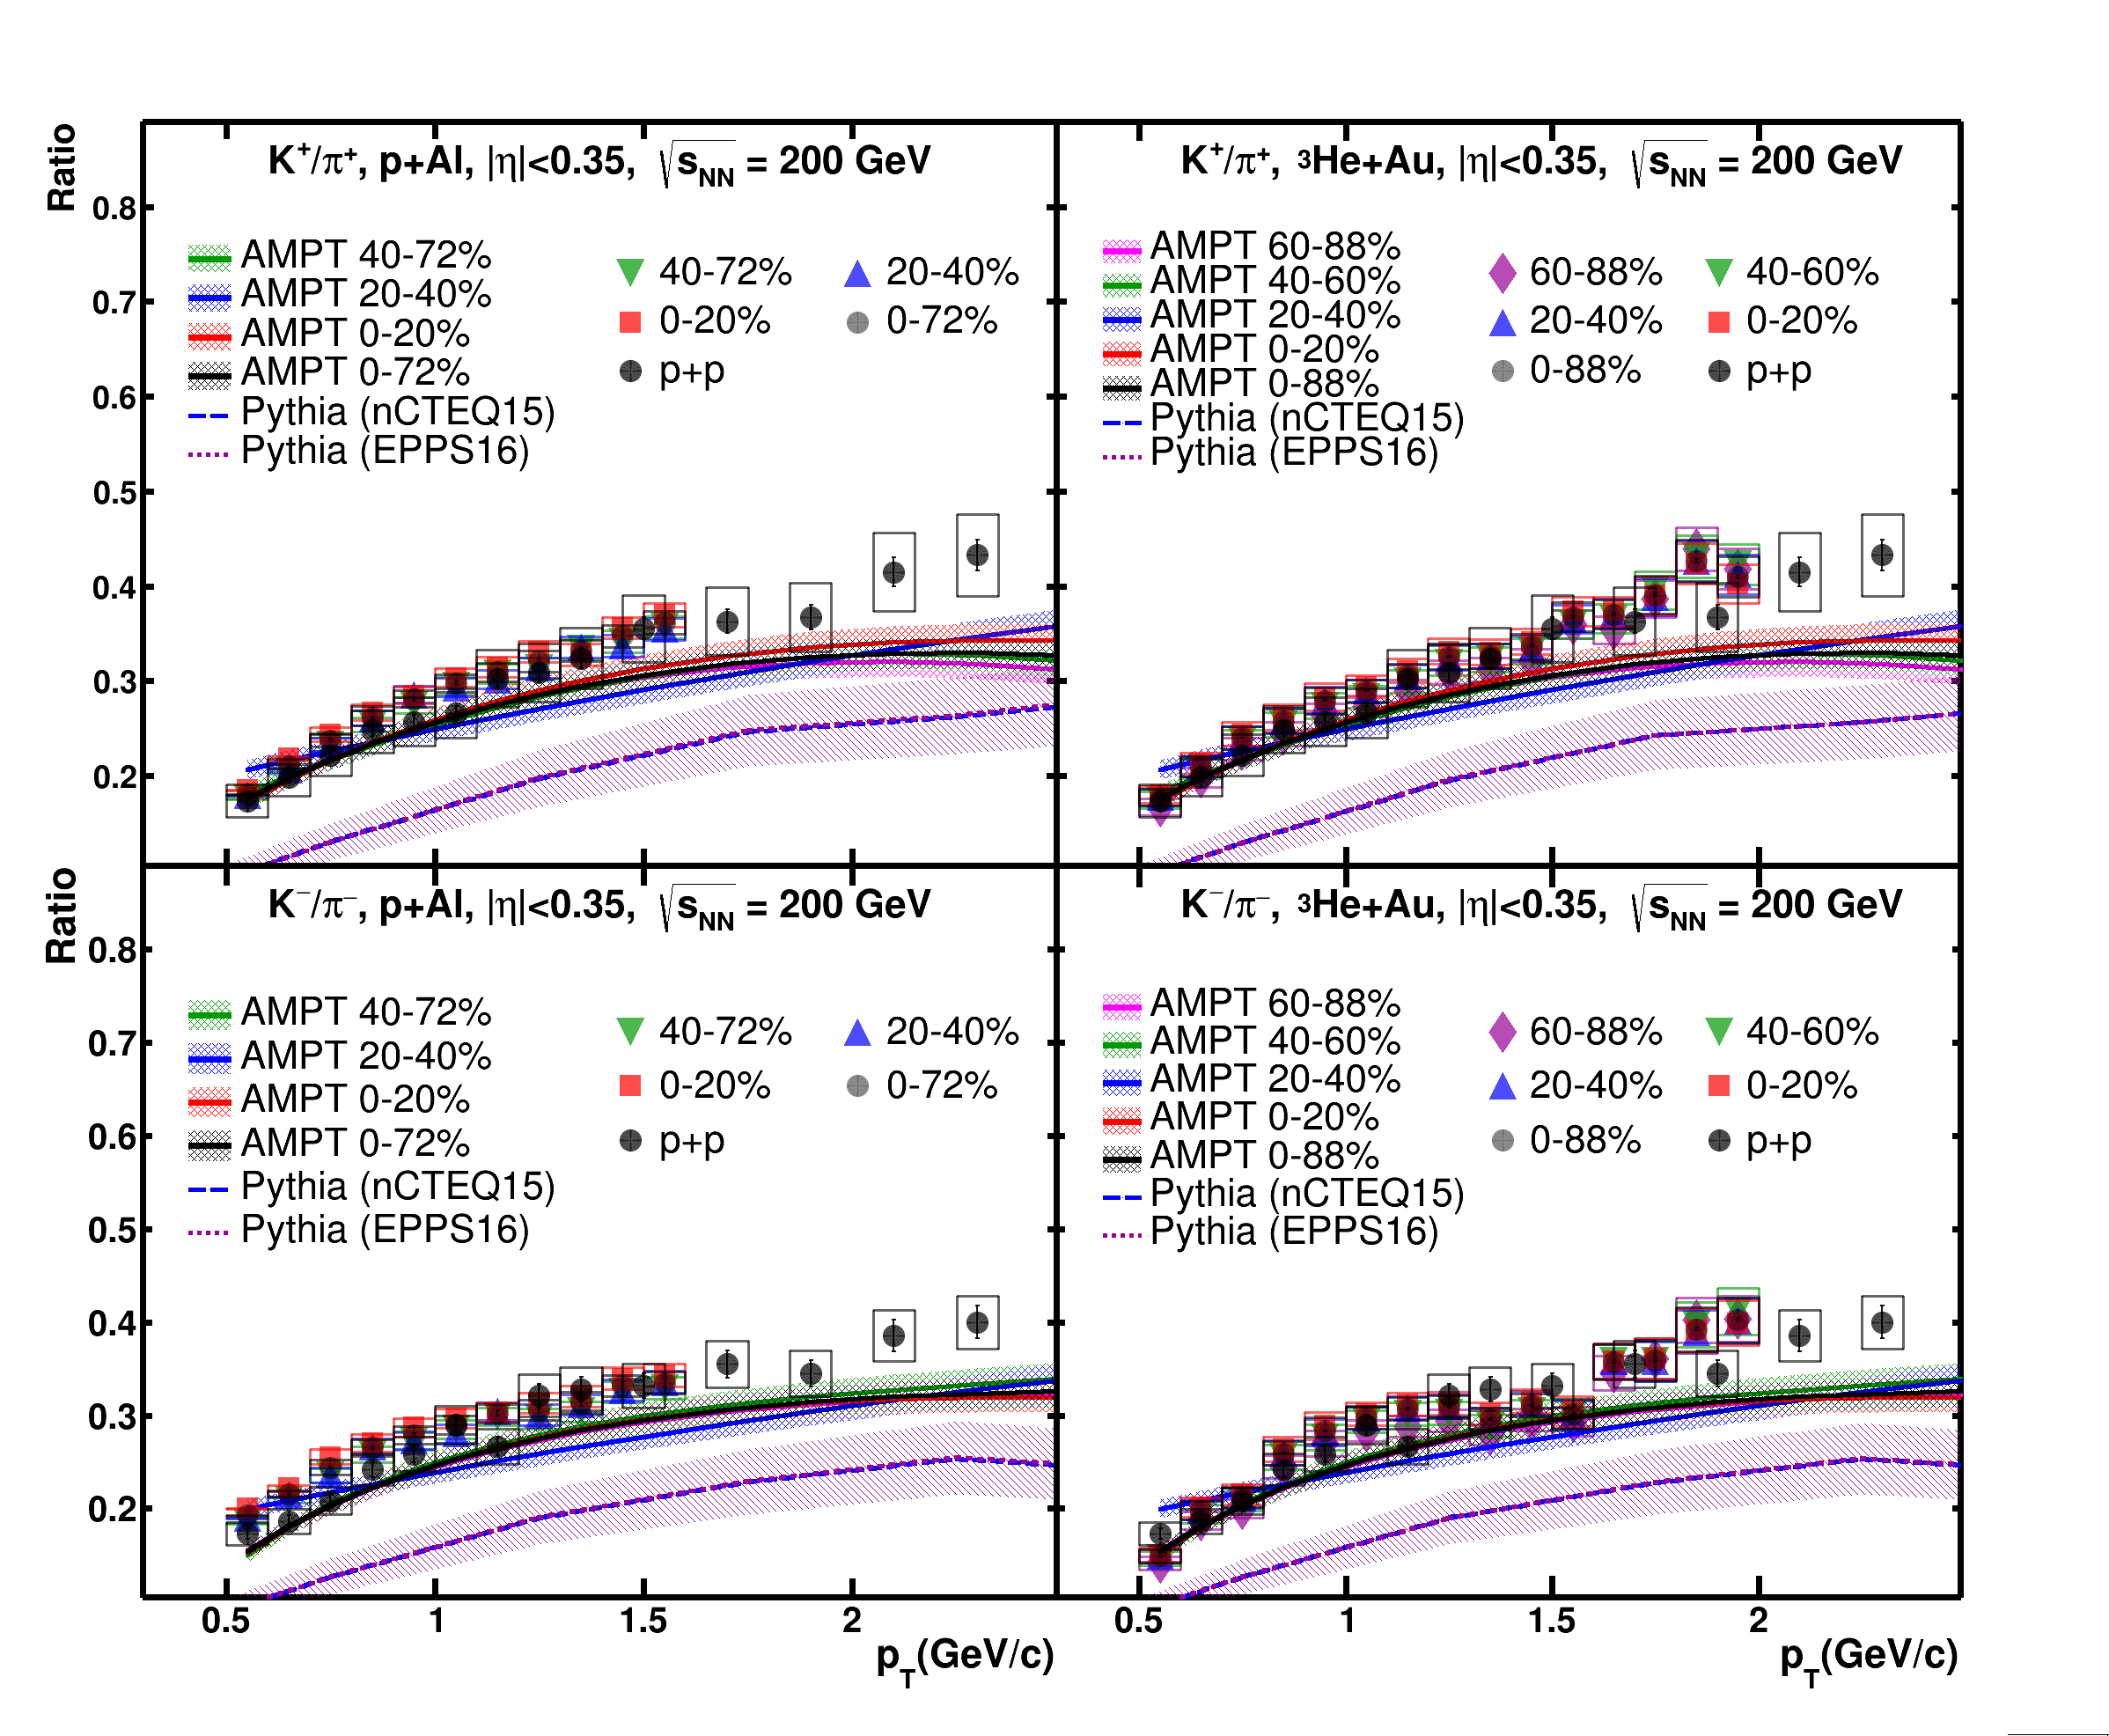
\includegraphics [width=0.7\linewidth]{Simulation/Ratios_AMPT_small_K2pi.png}
	\caption{Инвариантные спектры по поперечному массе, измеренные для отрицательно заряженных адронов в различных центральностях \pal, \heau, Cu+Au и U+U столкновениях.} 
	\label{img:synops_Ratio_SmallK2PI_sym}
\end{figure}


\FloatBarrier
\pdfbookmark{Заключение}{conclusion}                                  % Закладка pdf
В \underline{\textbf{заключении}} приведены основные результаты работы, которые заключаются в следующем:
%% Согласно ГОСТ Р 7.0.11-2011:
%% 5.3.3 В заключении диссертации излагают итоги выполненного исследования, рекомендации, перспективы дальнейшей разработки темы.
%% 9.2.3 В заключении автореферата диссертации излагают итоги данного исследования, рекомендации и перспективы дальнейшей разработки темы.
Представлены измерения инвариантных спектров по поперечному импульсу, факторов ядерной модификации, измеренные для идентифицируемых заряженных адронов ($\pi^\pm$, $K^\pm$, $p$, $\bar{p}$), а также отношений выходов адронов -- \pim/\pip, \Km/\Kp, \prot/\aprot, \prot/\pip, \aprot/\pim, \Kp/\pip, \Km/\pim.

На основе анализа инвариантных \pt \ и \mt \ спектров были получены значения температуры химического вымораживания $T_{0}$ и средней скорости коллективного потока частиц $\left< u_T \right>$ как функций от количества нуклонов-участников \Npart.
Величина $T_{0}\approx170$ МэВ и является постоянной относительно значений \Npart, в то время как величина \ut \ увеличивается с увеличением значений \Npart. Данный результат может свидетельствовать о том, что в столкновениях, характеризующихся большими значениями $\left<N_{part}\right>$ (центральные Cu+Au, Au+Au, U+U столкновения), коллективные эффекты выражены сильнее, чем в столкновениях с малыми значениями $N_{part}$ (\pal, \heau \ столкновения).

Сравнение факторов ядерной модификации идентифицированных заряженных адронов показало, что значения \rab, измеренные в системах с разной геометрией (\dau, \heau, Cu+Au, Au+Au и U+U) совпадают при одинаковых значениях \Npart.
Сделан вывод, что рождение идентифицированных заряженных адронов не зависит от геометрии и размера системы столкновения и определяется лишь размером области перекрытия ядер, характеризующейся значением \Npart.

В центральных столкновениях \heau, Cu+Au, U+U был обнаружен эффект увеличенного выхода протонов и антипротонов, что может быть объяснено доминированием вклада процессов рекомбинации в образовние иднентифицируемых заряженных адронов в диапазоне малых и промежуточных поперечных импульсов ($p_{T}<4$ ГэВ/$c$). 
В \pal \ столкновениях, а также в периферических столкновениях \heau, Cu+Au, U+U эффект увеличенного выхода протонов и антипротонов не наблюдался, что может быть интерпретировано как доминирование вклада процессов фрагментации в образовние иднентифицируемых заряженных адронов в диапазоне промежуточных поперечных импульсов (2 ГэВ/$c$ $<p_{T}<4$ ГэВ/$c$).

Полученные значения инвариантных спектров заряженных адронов могут быть использованы для уточнения параметров теоретических моделей, реализованных в пакетах прикладных программ, таких как  AMPT, HIJING, PHSD и др. В частности, для уточнения радиуса рекомбинации в рекомбинационных моделях, реализованных в таких программных пакетах как AMPT, PHSD.

\pdfbookmark{Литература}{bibliography}                                % Закладка pdf

\ifdefmacro{\microtypesetup}{\microtypesetup{protrusion=false}}{} % не рекомендуется применять пакет микротипографики к автоматически генерируемому списку литературы
\urlstyle{rm}                               % ссылки URL обычным шрифтом
\ifnumequal{\value{bibliosel}}{0}{% Встроенная реализация с загрузкой файла через движок bibtex8
    \renewcommand{\bibname}{\large \bibtitleauthor}
    \nocite{*}
    \insertbiblioauthor           % Подключаем Bib-базы
    %\insertbiblioexternal   % !!! bibtex не умеет работать с несколькими библиографиями !!!
}{% Реализация пакетом biblatex через движок biber
    % Цитирования.
    %  * Порядок перечисления определяет порядок в библиографии (только внутри подраздела, если \insertbiblioauthorgrouped).
    %  * Если не соблюдать порядок "как для \printbibliography", нумерация в \insertbiblioauthor будет кривой.
    %  * Если цитировать каждый источник отдельной командой --- найти некоторые ошибки будет проще.
    %
    %% authorvak
   \nocite{physica2020}%vak
   \nocite{physica2021}%vak
   \nocite{icppa2020}%vak
   \nocite{lomcon2021}%vak
   \nocite{nucleus2020}%vak    
   \nocite{ICPPA2022}

    \ifnumgreater{\value{usefootcite}}{0}{
        \begin{refcontext}[labelprefix={}]
            \ifnum \value{bibgrouped}>0
                \insertbiblioauthorgrouped    % Вывод всех работ автора, сгруппированных по источникам
            \else
                \insertbiblioauthor      % Вывод всех работ автора
            \fi
        \end{refcontext}
    }{
        \ifnum \totvalue{citeexternal}>0
            \begin{refcontext}[labelprefix=A]
                \ifnum \value{bibgrouped}>0
                    \insertbiblioauthorgrouped    % Вывод всех работ автора, сгруппированных по источникам
                \else
                    \insertbiblioauthor      % Вывод всех работ автора
                \fi
            \end{refcontext}
        \else
            \ifnum \value{bibgrouped}>0
                \insertbiblioauthorgrouped    % Вывод всех работ автора, сгруппированных по источникам
            \else
                \insertbiblioauthor      % Вывод всех работ автора
            \fi
        \fi
        %  \insertbiblioauthorimportant  % Вывод наиболее значимых работ автора (определяется в файле characteristic во второй section)
        \begin{refcontext}[labelprefix={}]
            \insertbiblioexternal            % Вывод списка литературы, на которую ссылались в тексте автореферата
        \end{refcontext}
        % Невидимый библиографический список для подсчёта количества внешних публикаций
        % Используется, чтобы убрать приставку "А" у работ автора, если в автореферате нет
        % цитирований внешних источников.
        \printbibliography[heading=nobibheading, section=0, env=countexternal, keyword=biblioexternal, resetnumbers=true]%
    }
}
\ifdefmacro{\microtypesetup}{\microtypesetup{protrusion=true}}{}
\urlstyle{tt}                               % возвращаем установки шрифта ссылок URL
